\vspace{-1em}
\section{The Internet}

\noindent
Terminology and concepts of the internet, which will be used throughout this text.

\begin{Def}[Protocol]

    A \textbf{protocol} is a set of rules which govern the exchange of data between devices. 
    Protocols define the format, timing, sequencing, and error control of data transmission \cite{rfc791}.
\end{Def}

\begin{Def}[Internet]

    The \textbf{Internet} is a global network of distributed system communicating over an \textbf{Internet Protocol} (IP) \cite{cloudflare_internet_protocol}.
    Documents served over the internet are referred to as \textbf{webpages} or \textbf{websites}.
\end{Def}
\begin{Def}[HTTP \& HTML]

    \textbf{HTTP} (HyperText Transfer Protocol), the protocol which transfer data over the internet, 
    distributing \textbf{HTML} (HyperText Markup Language) documents. Such 
    documents include \textbf{hyperlinks} to other websites, images, and other media \cite{rfc9110}.
\end{Def}
\begin{Def}[RFC (Request for Comments)]

    \textbf{RFC} (Request for Comments) is a publication from the \textbf{Internet Engineering Task Force} (IETF) 
    and the \textbf{Internet Society} (ISOC). This body governs the specifications for the internet and its protocols \cite{rfc}.
\end{Def}

\begin{Def}[DNS and IP Addresses]

    An \textbf{Internet Protocol address} (IP address) is a unique identifier for a device on a network. 
    The \textbf{Domain Name System} (DNS) maps domain names to IP addresses \cite{rfc760}.
\end{Def}

\newpage

\begin{Def}[Web Browser]

    A \textbf{web browser} is a software application for accessing the \textbf{World Wide Web} (WWW) \cite{ou_internet_history}.
\end{Def}

\begin{Def}[URL (Uniform Resource Locator)]

    A \textbf{URL} (Uniform Resource Locator) references each webpage, specifying protocol, domain, and path \cite{w3c_html_href_draft}.
    E.g., \texttt{http://www.example.com/path/to/resource}.
    \begin{itemize}
        \item \textbf{Protocol}: \texttt{http}
        \item \textbf{Domain}: \texttt{www.example.com}
        \item \textbf{Path}: \texttt{/path/to/resource}
    \end{itemize}
\end{Def}
\begin{Def}[Client-Server Model]

    Most of the internet operates on a \textbf{client-server model}, where an agent device--the \textbf{client}--requests data from another agent--the \textbf{server}--
    which serves an appropriate response. Clients are not servers and vice versa, as they receive and interpret data differently \cite{cloudflare_client_server}.
\end{Def}

\begin{Def}[HTTP Methods]
    
        When a client makes a request to a server, they must specify their intent, categorized by \textbf{HTTP methods} \cite{rfc2616}:
        \begin{itemize}
            \item \textbf{GET}: Retrieve data from the server.
            \item \textbf{POST}: Send data to the server.
            \item \textbf{PUT}: Update data on the server.
            \item \textbf{DELETE}: Remove data from the server.
        \end{itemize}
\end{Def}
\begin{Def}[HTTP Headers]

    \textbf{HTTP headers} are key-value pairs sent between the client and server to provide \textbf{metadata} about the request or response.
    \textbf{Metadata} is data about the transmitted data, telling the receiver how the incoming data should be interpreted \cite{rfc2616}.
\end{Def}


\newpage
\noindent
Tim Berners-Lee and his team at CERN developed the first web server and browser in 1989 \cite{w3c_http_history}.

\begin{table}[h!]
    \centering
    \begin{tabular}{@{}p{3cm}p{10cm}@{}}
    \toprule
    \textbf{HTTP Version} & \textbf{Description} \\ \midrule
    HTTP/0.9 (1991)       & Only supports GET method (retrieving HTML alone). \\
    HTTP/1.0 (1996)       & RFC\#1945, adding support for metadata in HTTP headers, status codes, and POST and HEAD methods \cite{rfc1945}. \\
    HTTP/1.1 (1997)       & Defined in RFC\#2068 and later updated by RFC\#2616, introduced persistent connections, chunked transfer encoding, and additional cache control mechanisms \cite{rfc2068}\cite{rfc2616}. \\
    HTTP/2 (2015)         & RFC\#7540, improving performance by enabling request and response multiplexing, header compression, and prioritization \cite{rfc7540}. \\
    HTTP/3 (2022)         & Builds upon HTTP/2's features and uses the QUIC transport protocol to reduce latency and improve security. \cite{rfc9114} \\ \bottomrule
    \end{tabular}
    \caption{Evolution of HTTP Versions}    
    \label{tab:http_versions}
\end{table}

\begin{Note}
    \textbf{Note:} In short, \textbf{Persistent Connections} allow multiple requests and responses to be sent over a single connection, reducing latency and improving performance \cite{rfc2616}.
    \textbf{Chunked Transfer Encoding} allows the server to send data in chunks, enabling the client to start processing data before the entire response is received \cite{rfc2616}.
    \textbf{Multiplexing}, is the ability to send multiple requests and responses over a single connection, reducing latency and improving performance \cite{multiplexing_networkencyclopedia}. 
     \textbf{QUIC} will be discussed alter on with other transfer protocols in a later section.

\end{Note}

\section{Data Transmission}
This section details how internet traffic is transmitted between devices.
\begin{Def}[ISO Model]

    The \textbf{ISO model} (International Organization for Standardization) is a conceptual framework for transmitted data between devices. 
    It is divided into seven layers of function\cite{ibm_osi_model}. Published in 1984 by the International Organization for Standardization (ISO) \cite{kanade_osi_model}.

\end{Def}
\begin{Def}[TCP/IP Model]

    The \textbf{TCP/IP model} (Transmission Control Protocol/Internet Protocol)
    is a concise representation of the ISO model used in practical settings \cite{yasar_tcpip}.
\end{Def}

\newpage


\begin{Def}[ISO Layers]

    \begin{enumerate}
        \item \textbf{Physical}: Converts data into physical signals (e.g., electrical, optical, or radio waves) for transmission across the network medium (e.g., cables, fiber optics, or wireless channels).
        \item \textbf{Data Link}: local delivery of directly connected devices within the same network.
        \item \textbf{Network}: Handles addressing, routing, in external networks from source to destination.
        \item \textbf{Transport}: Ensures end-to-end delivery, via a message delivery protocol.
        \item \textbf{Session}: Initiates and terminates network connections, ensuring efficient resource usage.
        \item \textbf{Presentation}: To translate, compress, and encrypt data  (e.g., Operating Systems).
        \item \textbf{Application}: User facing services such as, HTTP , FTP, DNS, SMTP, etc.
    \end{enumerate}
    \hfill \cite{leonard_osi_model}\cite{Rayes2022}
\end{Def}

\begin{Note}
    \textbf{Note:} Many of the above layers are closely related, if not identical. 
    In practice, layers 5-6 are integrated into layer 7, and 
    layers 1-2 are often combined into a single layer in the TCP/IP model.
    
\end{Note}


\begin{Def}[TCP/IP Layers]

    \begin{enumerate}
        \item \textbf{Network Interface}: Physical and data link layers from ISO. 
        \item \textbf{Internet}: Attaches IP addresses to data packets for routing across the internet.
        \item \textbf{Transport}: Defines the delivery protocol, segmenting data into packets.
        \item \textbf{Application}: The Session, Presentation, and Application layers from ISO.
    \end{enumerate}
    \hfill \cite{Rayes2022}
\end{Def}

Despite the numbering of the layers, the user interacts with the application layer, which communicates down the chain
of layers to the physical layer, where the data is transmitted over the network medium. The receiving device then 
interprets the data, moving back up the chain to the application layer.

\newpage 

\noindent
To illustrate the contrast between the ISO and TCP/IP models, consider the diagram:
\begin{figure}[h!]
    \centering
    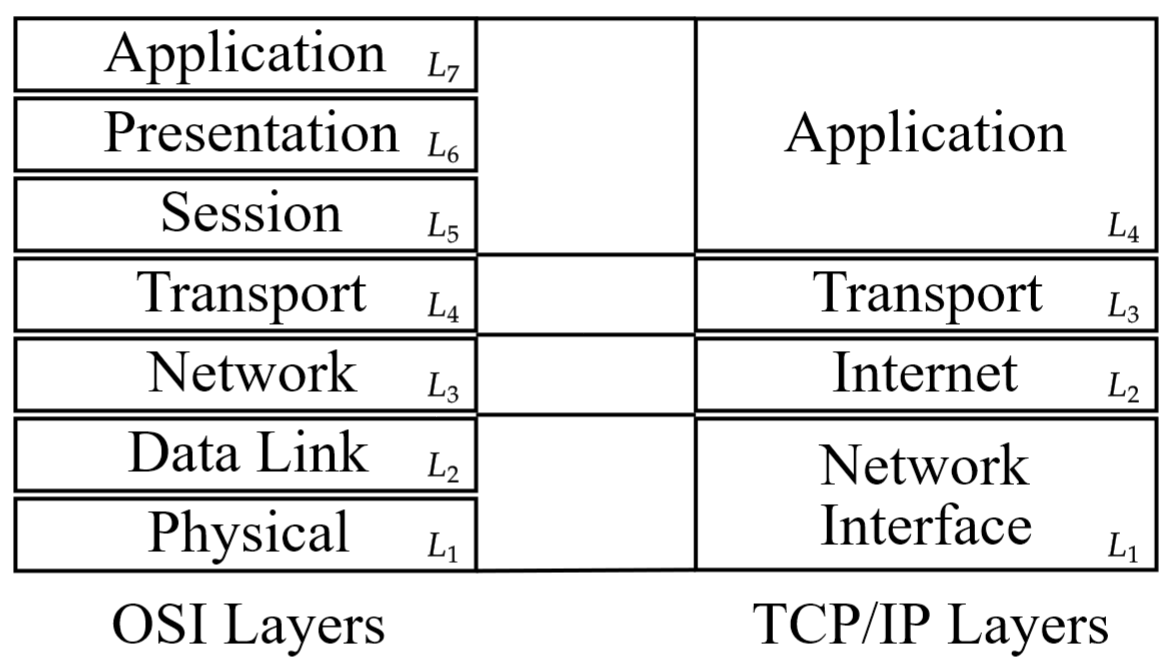
\includegraphics[width=0.7\textwidth]{Sections/network/osi_tcp.png}
    \caption{ISO vs TCP/IP Model}
    \label{fig:osi_tcpip}
\end{figure}

To illustrate two devices communicating over the internet, consider the diagram:

\section{Routing Networks}

\noindent
When IP addresses began


\begin{Def}[Routing]

    \textbf{Routing} is the process of selecting the best path across networks. 
    Data is segmented into packets, each with a destination address. 
    \textbf{Routers} are devices which forward this data through the network.

    Routers have a \textbf{routing table} which maps to other reachable networks. 
    When a packet arrives, the router checks against its routing table to find the best path.
    \hfill \cite{cloudflare_routing}
\end{Def}

\begin{Def}[Hop-by-Hop \& End-to-End Routing]

    \begin{itemize}
        \item  \textbf{Hop-by-Hop Routing}: When a packet of data is forwarded from one router to the next, a forward decision is called a \textbf{hop}.
        \item \textbf{End-to-End Routing}: The process of sending data from source to destination without intermediate hops.
    \end{itemize}
    \noindent
    It is often rare to see end-to-end routing in modern networks, as data is often forwarded through multiple routers. A target 
    destination may be unreachable from a given router.
    \hfill \cite{heimlicher_e2e_hbh}
\end{Def}

\newpage

\begin{Def}[Router Advertising]

    When routers inform each other of their existence and the networks they can reach \cite{narten_rfc4861}.
\end{Def}
\begin{Def}[Routing Protocols]
    
    \begin{itemize}
        \item \textbf{IP} (Internet Protocol): The primary protocol for routing data across the internet.
        \item \textbf{BGP} (Border Gateway Protocol): The protocol for routing data between \textbf{Autonomous Systems} (AS). 
        an AS is a collection of IP networks and routers under the control of a single entity (e.g., an \textbf{ISP} (Internet Service Provider)).
        These may only connect with each other if they have a mutual agreement. ASes identify themselves to 
        external networks using a unique \textbf{Autonomous System Number} (ASN).
        These are unique 16 bit numbers between 1-65534 or 32 bit numbers between 131072-4294967294 (e.g., \texttt{AS12345}) \cite{cloudflare_autonomous_system}.
        \item \textbf{OSPF} (Open Shortest Path First): A link-state routing protocol used within an AS. Link-state protocols are a set 
        of algorithms which determine the best path, based on the topology of a network graph \cite{kurose_link_state_routing}.
        It is also an \textbf{IGP} (Interior Gateway Protocol), meaning it operates within a single AS. It does so by sending out \textbf{LSAs} (Link State Advertisements) to other routers in the AS.
        Then routers in the system build a \textbf{LSADB} (Link State Advertisement Database) of the network topology. Then a shortest path algorithm is run to determine the best path to each network \cite{certbros_ospf_explained}.
        \item \textbf{RIP} (Routing Information Protocol): RIP employs hop count as a routing metric, with a maximum allowable hop count of 15 (network size limitation).
        It operates as an \textbf{IGP} within a single AS, periodically broadcasting the entire routing table to neighboring routers every 30 seconds,
        which can lead to slower convergence and higher bandwidth usage compared to other protocols. RIP is largely deprecated \cite{javatpoint_rip_protocol}.
    \end{itemize}
\end{Def}

\begin{Def}[IP Addressing]

    \textbf{IP addresses} are unique identifiers for devices on a network. 
    There are two versions of IP addresses, \textbf{IPv4} and \textbf{IPv6}.
    IPv4 A 32-bit address ($2^{32}$ addresses), employed since 1983, quickly exhausted all available addresses by the 2010s \cite{info12060246}.
    IPv6 is a 128-bit address ($2^{128}$ addresses), introduced in 1998 , in an attempt to address this shortage \cite{deering_ipv6_specification}\cite{ibm_ipv4_ipv6_formats}.
    For example,
    \begin{itemize}
        \item \textbf{IPv4}: a decimal octet ``$x.x.x.x$'': $x \in [0, 255]$ (e.g., \texttt{192.168.1.1}).
        \item \textbf{IPv6}: a hexadecimal segment ``$y:y:y:y:y:y:y:y$'': $y\in [0, FFFF]$ \\
         (e.g., \texttt{2001:0db8:85a3:0000:0000:8a2e:0370:7334}).
    \end{itemize}
\end{Def}

\newpage

\begin{Def}[Subnetting]

    Instead of a large monolith network of routers, networks can be divided into 
    smaller networks called \textbf{subnets}. I.e., Instead of passing data to every device on a network, routers forward data to a representative device on each subnet.
    \hfill \cite{cloudflare_subnet}
\end{Def}
\begin{Def}[Subnet Masking]

    A \textbf{subnet mask} defines which part of an IP address identifies the \textbf{network} and which part identifies the \textbf{host}.
\end{Def}
\begin{Def}[Classful Network]

    In the beginning, the first octet of an IPv4 address determined the network class---only allowing for 256 networks.
    The RFC\#791 published in 1981 introduced \textbf{Classful Networks} \cite{postel_internet_protocol}. 
    It uses the first three bits of the first octet's binary representation as a subnet mask to determine a class ranging from A-E---D and E were rarely if ever used.
\end{Def}

\begin{table}[h!]
    \centering
    \begin{tabular}{@{}p{.1cm}p{1.1cm}p{2cm}p{3cm}p{4cm}@{}}
    \toprule
    \textbf{Class} & \textbf{Binary Prefix} & \textbf{Range (Decimal)} & \textbf{Purpose} & \textbf{Details} \\ \midrule
    A              & \texttt{0xx}           & 1.0.0.0 to 126.0.0.0     & Unicast (large networks) & For large organizations; 8 bits for the network, 24 for hosts. \\
    B              & \texttt{10x}           & 128.0.0.0 to 191.255.0.0 & Unicast (medium networks) & For medium-sized networks; 16 bits for the network, 16 for hosts. \\
    C              & \texttt{110}           & 192.0.0.0 to 223.255.255.0 & Unicast (small networks) & For small networks; 24 bits for the network, 8 for hosts. \\
    D              & \texttt{1110}          & 224.0.0.0 to 239.255.255.255 & Multicast & Reserved for multicast addressing; not for general use. \\
    E              & \texttt{1111}          & 240.0.0.0 to 255.255.255.255 & Experimental and future use & Reserved for research and development; not assigned for standard use. \\ \bottomrule
    \end{tabular}
    \caption{Overview of IPv4 Address Classes}
    \label{tab:ipv4_classes}
\end{table}






\newpage 

\noindent 

\begin{Def}[Fixed Length Subnet Masking (FLSM)]

    \textbf{Fixed Length Subnet Masking} (FLSM) is a technique which divides a network into equal-sized subnets. This
    may lead to inefficient use of IP addresses.
    \hfill \cite{awati_vlsm}
\end{Def}
\begin{Def}[Variable Length Subnet Masking (VLSM)]

    \textbf{Variable Length Subnet Masking} (VLSM) is a technique which allows for the creation of subnets with different sizes. 
    As some ASes may require more IP addresses than others, VLSM allows for more efficient use of IP addresses.
    \hfill \cite{awati_vlsm}
\end{Def}
\noindent

\begin{Def}[Classless Inter-Domain Routing (CIDR)]

    \textbf{CIDR}, introduced in 1993 through RFC\#1518 and RFC\#1519 to address IPv4 exhaustion.
    \textbf{CIDR replaced classful subnetting} with VLSM \cite{fuller_cidr_rfc1519}.

    \noindent
    CIDR denoted as \underline{\texttt{IP Address/Prefix Length} (e.g., \texttt{192.168.1.0/24})}, where:
    \begin{itemize}
        \item \texttt{IP Address}: Represents the starting address of the network.
        \item \texttt{Prefix Length}: The number of bits used for the \textbf{network portion} of the address. E.g.,
    \end{itemize}

        \vspace{-1em}
        \begin{center}
            \large
            \texttt{255.0.0.0\textbf{/8}}; \hspace{.2em} \texttt{255.255.0.0\textbf{/16}}; \hspace{.2em} \texttt{255.255.255.0\textbf{/24}}; \hspace{.2em} \texttt{255.255.255.192\textbf{/26}};
            \normalsize
        \end{center}
\end{Def}

\begin{Def}[Route Aggregation]

    CIDR introduced \textbf{Route Aggregation} also known as \textbf{Supernetting}, or \textbf{Route Summarization}, is the process of combining multiple routes into a single route advertisement.
    \textbf{Example}:
    Consider an organization assigned the following contiguous IP address blocks:
    \begin{center}
        \texttt{192.168.\textbf{1}.0/24}; \quad \texttt{192.168.\textbf{2}.0/24}; \quad \texttt{192.168.\textbf{3}.0/24}; \quad \texttt{192.168.\textbf{4}.0/24};
    \end{center}
    Each block holding 256 IP addresses with a subnet mask of 255.255.255.0, requiring four routing table entries. 
    However, these networks share a common prefix: the first 22 bits (\texttt{192.168.0.0/22}), which aggregates to: \texttt{\textbf{192.168.0.0/22}} \cite{fuller_cidr_rfc1519}.

\end{Def}
\begin{theo}[Routers - Path of Least Resistance]

    If the target address of a router is \texttt{192.168.1.5}
    and the router has routes, \texttt{192.168.0.0/16} vs. \texttt{192.168.1.0/24}, the prefix length 24 will be chosen.
\end{theo}
\newpage
\begin{Def}[IP Address Components]
    
        \item \textbf{Network Address}:
        \begin{itemize}
            \item Identifies the specific network segment to which a device is connected.
            \item Determined by setting all bits in the host portion to 0.
            \item Example: For the IP address \texttt{192.168.1.10} with a subnet mask of \texttt{255.255.255.0} (/24), the network address is \texttt{192.168.1.0}.
        \end{itemize}

        \item \textbf{Host Address}:
        \begin{itemize}
            \item Uniquely identifies a device within a network segment.
            \item The bits in the IP address designated for hosts, specified by the subnet mask.
            \item Example: In the IP address \texttt{192.168.1.10} with a /24 subnet mask, the host portion is the last octet (10).
        \end{itemize}

        \item \textbf{Broadcast Address}:
        \begin{itemize}
            \item Used to communicate with all devices on a specific network segment simultaneously.
            \item Determined by setting all bits in the host portion to 1.
            \item Example: For the network \texttt{192.168.1.0/24}, the broadcast address is \texttt{192.168.1.255}.
        \end{itemize}
      

    \hfill \cite{sunshine_rfc919} \cite{postel_rfc922} \cite{manning_rfc1878}

\end{Def}
\noindent
Consider the IP address \texttt{192.168.2.12/26} and its binary \texttt{11000000.10101000.00000010.00001100}:

\vspace{-1em}
\begin{figure}[h!]
    \hspace{2em}
    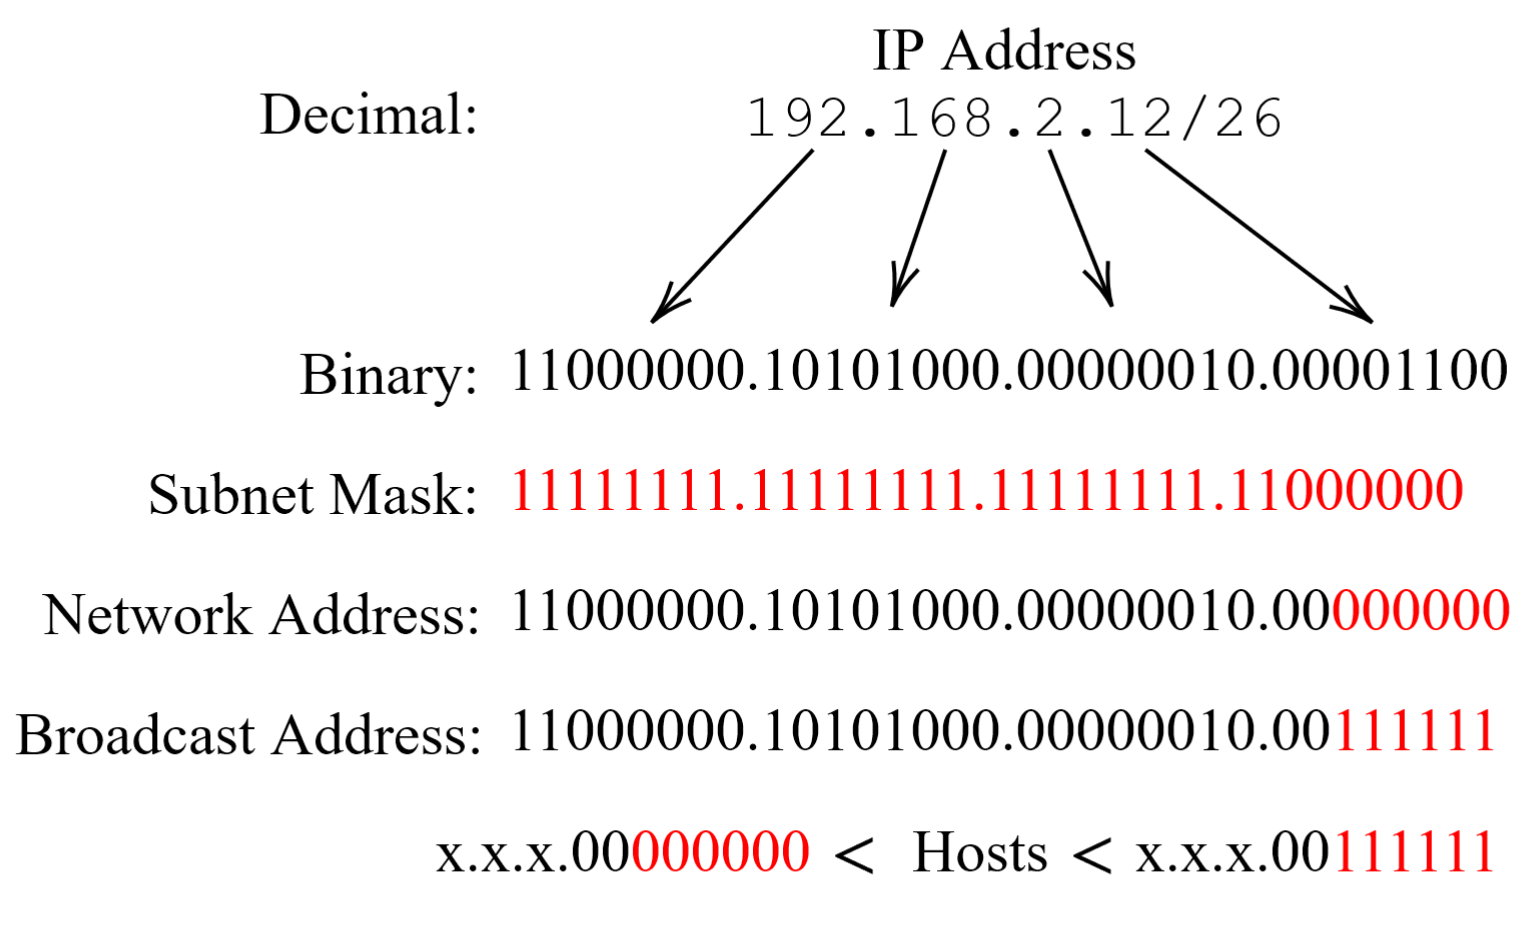
\includegraphics[width=0.7\textwidth]{Sections/network/ip_address.png}
    \caption{Binary Subnetting: Red indicating parts of the IP address identified for each component.}
    \label{fig:subnetting}
\end{figure}
\noindent
\begin{Def}[Common Types of Area Networks (ANs)]

    \textbf{PAN (Personal Area Network)}: A network for personal devices, such as smartphones, smartwatches, or earbuds, with a short range (typically a few meters) using technologies like Bluetooth or infrared.\\

    \noindent
    \textbf{LAN (Local Area Network)}: Connects devices within a small area, such as a home, office, or school, enabling high-speed communication and resource sharing.\\

    \noindent
    \textbf{WLAN (Wireless Local Area Network)}: A wireless version of LAN that uses Wi-Fi to connect devices within a localized area like a home or office.\\

    \noindent
    \textbf{CAN (Campus Area Network)}: A network that connects multiple LANs across a limited geographical area, such as a university campus or corporate facility, for resource sharing and communication.\\

    \noindent
    \textbf{MAN (Metropolitan Area Network)}: Covers a larger area than a LAN, typically a city or metropolitan region, connecting multiple LANs or CANs via high-speed infrastructure like fiber optics.\\

    \noindent
    \textbf{WAN (Wide Area Network)}: Connects LANs, MANs, or other networks over large geographical areas, such as countries or continents. The internet is the largest WAN example.\\

    \noindent
    \textbf{SAN (Storage Area Network)}: A high-speed network that provides access to storage devices for data centers, ensuring fast and reliable storage management.\\

    \noindent
    \textbf{EPN (Enterprise Private Network)}: A private network created by organizations to connect their various locations securely, often including VPNs for remote access.\\

    \noindent
    \textbf{VPN (Virtual Private Network)}: Creates a secure, encrypted connection over public networks, like the internet, to allow users to access private networks remotely.\\

    \noindent
    \textbf{HAN (Home Area Network)}: A network within a home environment, connecting personal devices like computers, printers, and smart home gadgets.\\

    \noindent
    \textbf{GAN (Global Area Network)}: A large-scale network that connects multiple WANs and supports worldwide communication, with the internet as its most prominent example.

    \hfill \cite{petryschuk_types_of_networks}
\end{Def}

\newpage 

\begin{Example}[Subnetting a Network via VLSM]


Consider the FLSM below, which all have 62 hosts per network:
\[
\begin{array}{|c|c|c|}
\hline
\textbf{Network Address} & \textbf{Hosts} & \textbf{Broadcast Address} \\ \hline
192.168.100.0 & .1 - .62 & .63 \\ \hline
192.168.100.64 & .65 - .126 & .127 \\ \hline
192.168.100.128 & .129 - .190 & .191 \\ \hline
192.168.100.192 & .193 - .254 & .255 \\ \hline
\end{array}
\]
\noindent
Below illustrates this network, where a router of base address \texttt{192.168.1.0/24},
connects four LANs:\\

\hspace{4em}
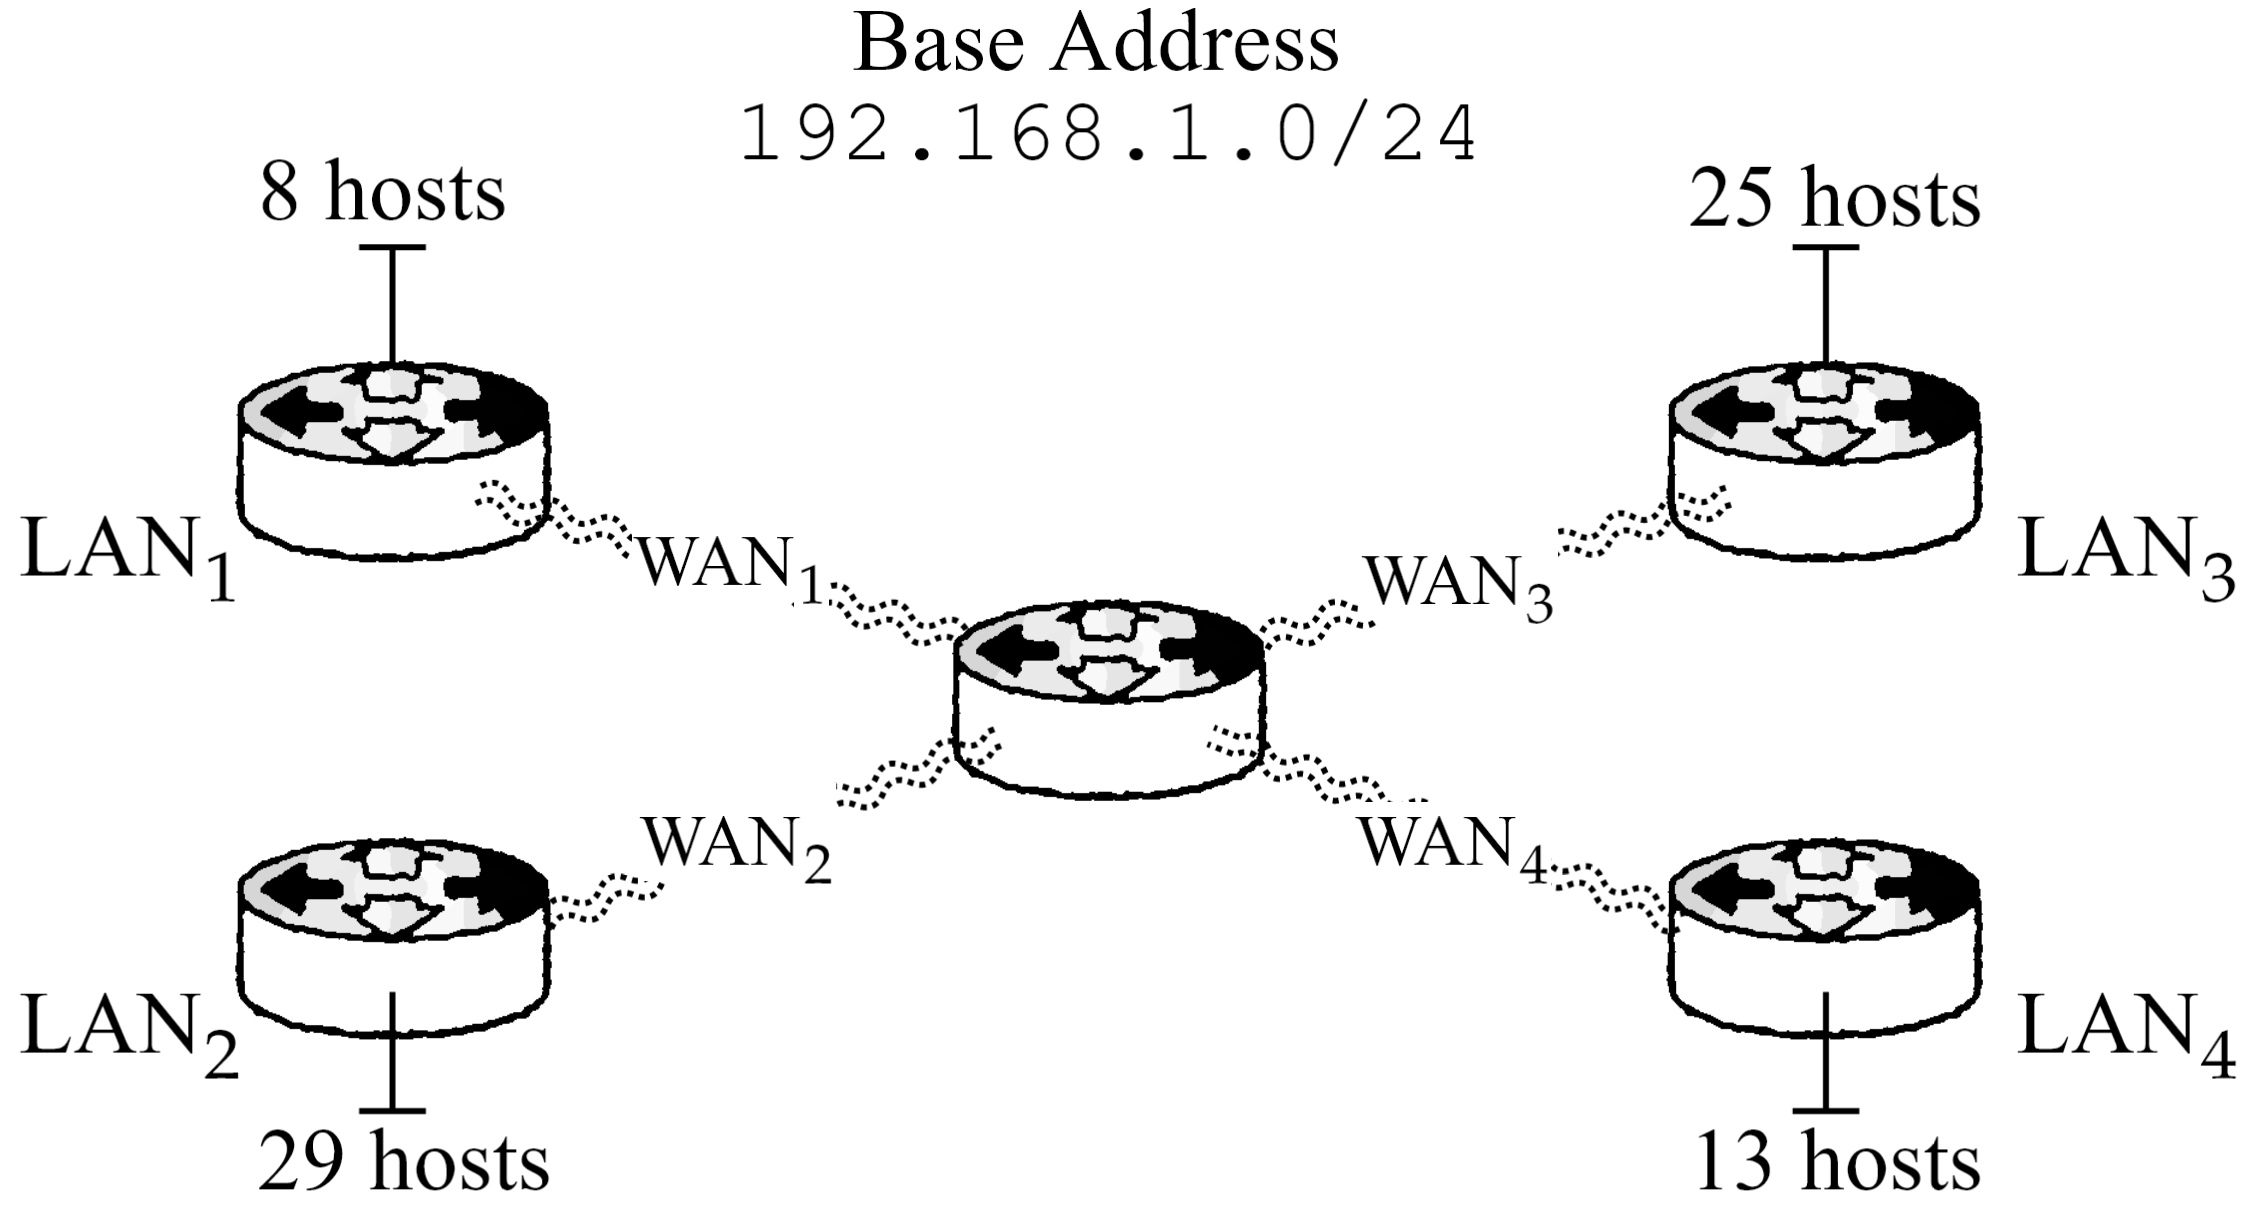
\includegraphics[width=0.7\textwidth]{Sections/network/subnetting.png}\\

\noindent
\textbf{Subnetting:} Process each LAN from largest to smallest, Select the nearest block size, identify the network, host, and broadcast addresses.
Since there is a subnet mask of /24, blocks $[128, 64, 32, 16, 8, 4, 2, 1]$ are available. This is the case as 
$2^8 = 256$. If a LAN has 129 hosts, that LAN will occupy all 256 addresses.\\
\begin{enumerate}
    \item \textbf{LAN$_2$}: 29 hosts $\Rightarrow$ Block size 32. Network: \texttt{x.0}, Broadcast: \texttt{x.31}, Hosts: \texttt{x.1-x.30}.
    \item \textbf{LAN$_3$}: 25 hosts $\Rightarrow$ Block size 32. Network: \texttt{x.32}, Broadcast: \texttt{x.63}, Hosts: \texttt{x.33-x.62}.
    \item \textbf{LAN$_4$}: 13 hosts $\Rightarrow$ Block size 16. Network: \texttt{x.64}, Broadcast: \texttt{x.79}, Hosts: \texttt{x.65-x.78}.
    \item \textbf{LAN$_1$}: 8 hosts $\Rightarrow$ Block size 16. Network: \texttt{x.80}, Broadcast: \texttt{x.95}, Hosts: \texttt{x.81-x.94}.
\end{enumerate}

\noindent
8 hosts need occupy 16, as a block size of 8 only has 6 usable addresses. The computed subnet now only occupies addresses 
\texttt{x.0-x.95}, leaving room for additional LANs \cite{eastcharmer_vlsm_subnetting}. 

\end{Example}
    
\newpage 

\begin{Def}[Ports]

    A host may have serve multiple resources, HTTP, FTP, SSH, etc. \textbf{Ports} are used to distinguish between these services.
    Port numbers are managed by the \textbf{Internet Assigned Numbers Authority (IANA)}, outlined in RFC\#6335. The RFC divides ports into three categories:
    \begin{itemize}
        \item \textbf{Well-Known Ports (0–1023)}: Reserved for standardized services (HTTP: port 80).
        \item \textbf{Registered Ports (1024–49151)}: User applications or services upon request.
        \item \textbf{Dynamic/Private Ports (49152–65535)}: Temporary communications. \hfill \cite{rfc6335}
    \end{itemize}
    \noindent
    Which can be found here: \href{https://www.iana.org/assignments/service-names-port-numbers/service-names-port-numbers.xhtml}{IANA Service Names and Port Numbers}.
\end{Def}

\vspace{-.25em}
\begin{Def}[Transport Layer Protocols (TCP, UDP, QUIC)]

    Out of numerous transport layer protocols, there are three primary protocols used to dictate the flow of data between devices:
    \begin{itemize}
        \item \textbf{TCP}: A connection-oriented protocol that ensures reliable communication by establishing a connection before transmitting data. TCP guarantees delivery, maintains packet order, and retransmits lost packets. It is ideal for applications like web browsing (HTTP/HTTPS) and file transfers (FTP). \hfill \cite{rfc793}
        \item \textbf{UDP}: A connectionless protocol that prioritizes speed by sending data without establishing a connection. It does not guarantee delivery, order, or error correction, making it suitable for time-sensitive applications like video streaming, online gaming, and DNS lookups. \hfill \cite{rfc768}
        \item \textbf{QUIC}: A modern, connection-oriented protocol built on UDP that combines speed with reliability. QUIC provides features like multiplexed streams, faster connection establishment, and built-in encryption, addressing TCP's latency issues while retaining UDP's efficiency. It is optimized for HTTP/3 and increasing in use. \hfill \cite{rfc9000}
    \end{itemize}
\end{Def}

\begin{Def}[MAC Address]

    A \textbf{MAC address} (Media Access Control address) is a globally unique identifier assigned to a device's network interface card (NIC) at the \textbf{network interface layer} of the TCP/IP model. 
    MAC addresses consist of 48 bits, typically represented as six pairs of hexadecimal digits\\
    (e.g., \texttt{00:1A:2B:3C:4D:5E}).

    The first 24 bits represent the \textbf{Organizationally Unique Identifier (OUI)}, assigned to manufacturers by the \textbf{Institute of Electrical and Electronics Engineers (IEEE)}.
    The remaining 24 bits are left to the manufacturer to ensure device uniqueness \cite{ieee8022001}.
\end{Def}
    

\begin{Def}[Ethernet]

    \textbf{Ethernet} is a protocol used at the \textbf{network interface layer} of the TCP/IP model for communication within local area networks (LANs).
    If a network is communicating at these layers—such as in homes, offices, or data centers—Ethernet provides the rules for framing, addressing, and transmitting data between devices using \textbf{MAC addresses}. 
    Ethernet is the dominant standard for wired LAN communication. \hfill \cite{9844436}

\end{Def}

\vspace{-1em}
\begin{figure}[h]
    \hspace{1em}
    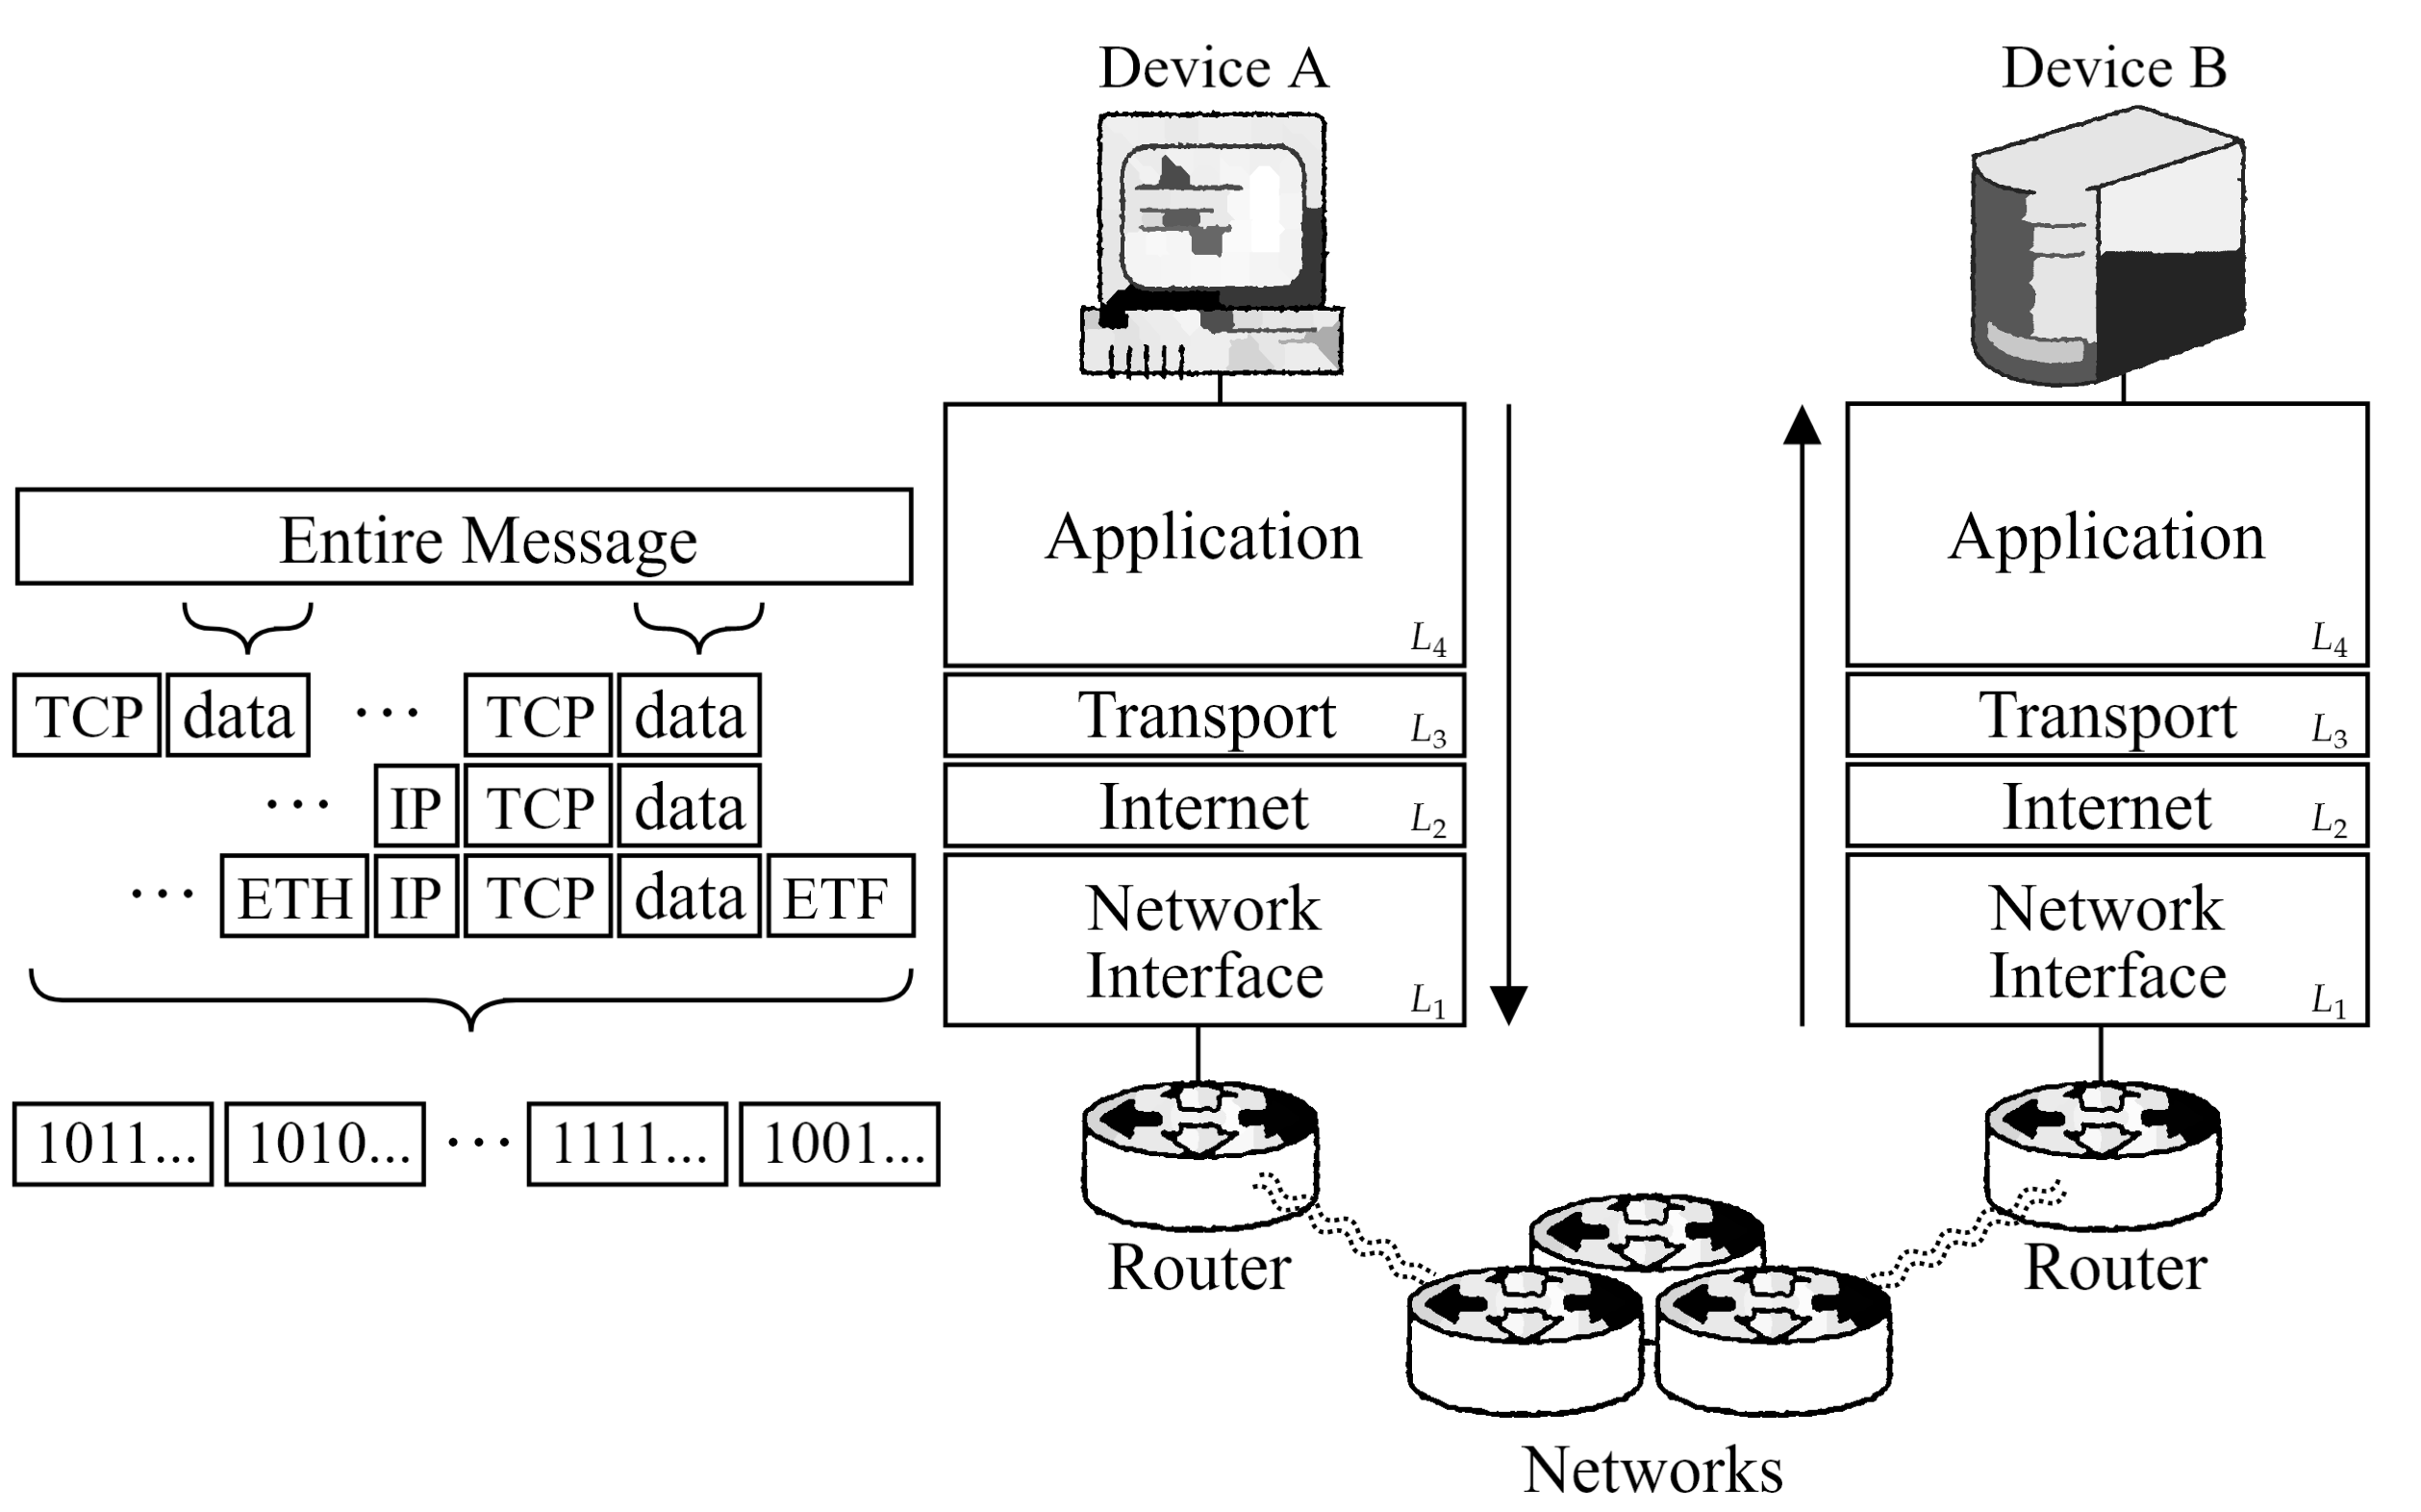
\includegraphics[width=0.9\textwidth]{Sections/network/tcpip.png}
    \caption{Data transmission between devices from application to physical layer and back.}
    \label{fig:tcpip}
\end{figure}

\begin{enumerate}
    \item \textbf{Transport Layer (L3)}: Data is segmented and encapsulated by a protocol like TCP, UDP, or QUIC. Headers with source and destination port numbers are added to enable communication with the correct application.
    
    \item \textbf{Network Layer (L2)}: Data is encapsulated into an IP packet, including the source and destination IP addresses. The router uses the destination IP to determine if the packet should be sent locally or to a remote network.

    \item \textbf{Data Link Layer (L1)}: For local delivery, the packet is encapsulated into an Ethernet frame with source and destination MAC addresses. If the packet is leaving the local network, it is sent to the router. Data is wrapped with a \textbf{Ethernet Header and Trailer}.

    \item \textbf{Routing Across Networks}: If the destination is on another network, routing protocols like \textbf{BGP} or \textbf{OSPF} determine the optimal path. The packet is forwarded across multiple routers, each stripping the current Ethernet frame and applying a new one for the next hop.
\end{enumerate}
\newpage

\begin{Def}[TCP Header]

    A \textbf{TCP header}, as defined in RFC\#793, is a component of a TCP segment that contains essential information for reliable data delivery between devices. 
    Minimum size of 20 bytes and a max 60 bytes with options. It's called a header as it sits \textit{ahead} of the \textbf{payload} (data) in the segment. Eg., [TCP Header (20–60 bytes), Payload (0-65,495 bytes)].
\hfill \cite{rfc793}
\end{Def}

\begin{table}[h]
    \centering
    \resizebox{1\textwidth}{!}{
    \begin{tabular}{|l|c|p{7cm}|}
    \hline
    \textbf{Field}                & \textbf{Size (bits)} & \textbf{Description} \\ \hline
    Source Port                  & 16                  & Identifies the sending application on the source device. \\ \hline
    Destination Port             & 16                  & Identifies the receiving application on the destination device. \\ \hline
    Sequence Number              & 32                  & Specifies the position of the first byte of data in the current segment relative to the start of the data stream. \\ \hline
    Acknowledgment Number        & 32                  & Used to confirm receipt of data by specifying the next expected byte. \\ \hline
    Data Offset                  & 4                   & Indicates the size of the TCP header in 32-bit words. \\ \hline
    Reserved                     & 6                   & Reserved for future use; must be set to 0. \\ \hline
    Flags (Control Bits)         & 6                   & Includes control flags (e.g., SYN, ACK, FIN) for managing connections and flow. \\ \hline
    Window Size                  & 16                  & Specifies the size of the sender's receive window for flow control. \\ \hline
    Checksum                     & 16                  & Ensures the integrity of the TCP header and payload. \\ \hline
    Urgent Pointer               & 16                  & Points to urgent data within the segment, if the URG flag is set. \\ \hline
    Options                      & Variable            & Optional fields for additional settings (e.g., Maximum Segment Size). \\ \hline
    Padding                      & Variable            & Ensures the header is a multiple of 32 bits. \\ \hline
    \end{tabular}
    }
    \caption{Fields of the TCP Header}
    \label{tab:tcp-header}
\end{table}

\begin{Def}[Maximum Transmission Unit (MTU)]

    The \textbf{Maximum Transmission Unit (MTU)} is the maximum size of a packet, in bytes,
    that a network can receive before requiring further fragmentation. Theoretically, a payload 
    of 65,535 bytes can be sent, but in practice, are much lower (e.g., Ethernet 1,500 bytes). \cite{rfc894}\cite{rfc1191}
    
\end{Def}
    
\newpage

\vfill
\begin{figure}[h!]
    \hspace{-2.5em}
    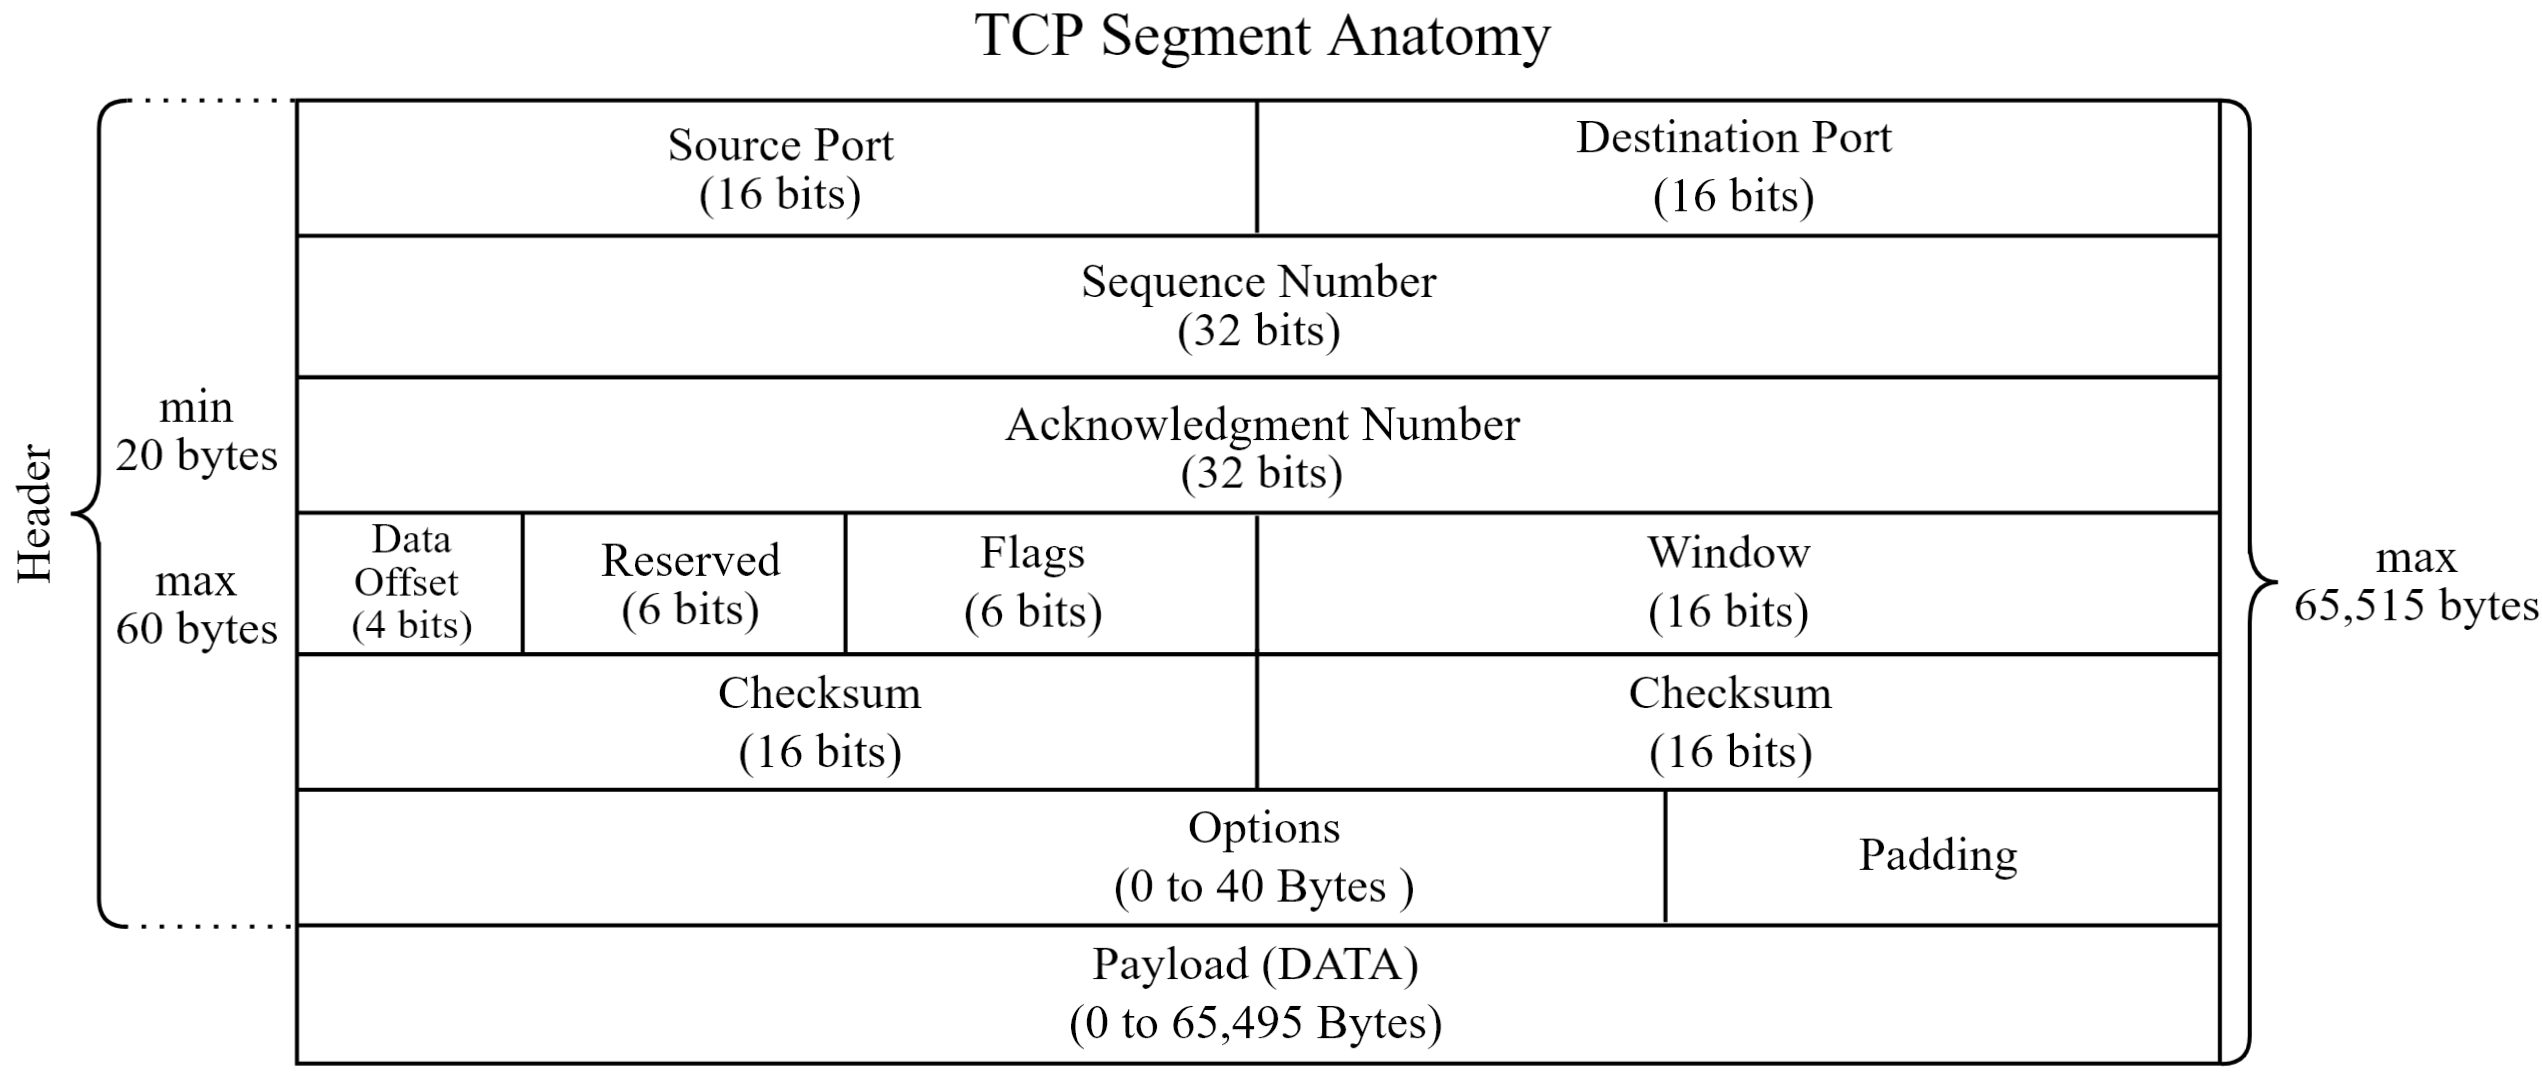
\includegraphics[width=1.1\textwidth]{Sections/network/segment.png}
    \caption{TCP Header}
    \label{fig:tcp_header}
\end{figure}

\vfill
\begin{Def}[Flags (Control Bits) in TCP Header]

    The \textbf{Flags (Control Bits)} in the TCP header are a 6-bit field used to control and manage the state of a TCP connection. Each bit represents a specific flag, and one or more flags can be set simultaneously to define the segment's purpose.
    
    \textbf{List of Control Bits}:
    \begin{itemize}
        \item \textbf{URG (Urgent Pointer)}: Indicates that the Urgent Pointer field is significant.
        \item \textbf{ACK (Acknowledgment)}: Confirms receipt of data; the Acknowledgment Number field is valid.
        \item \textbf{PSH (Push Function)}: Requests the receiver to pass the data to the application immediately.
        \item \textbf{RST (Reset)}: Resets the connection due to errors or unexpected conditions.
        \item \textbf{SYN (Synchronize)}: Initiates a connection by synchronizing sequence numbers.
        \item \textbf{FIN (Finish)}: Signals the sender's intention to terminate the connection.
    \end{itemize}
    
    \hfill \cite{rfc793}
\end{Def}

\newpage
\begin{Def}[TCP Options]

    \begin{itemize}
        \item \textbf{Maximum Segment Size (MSS)}: Specifies the largest segment size the sender is willing to accept (4 bytes).
        \item \textbf{Window Scale}: Extends the window size field to support larger flow control (3 bytes).
        \item \textbf{Selective Acknowledgment (SACK)}: Allows acknowledgment of specific data blocks, improving performance in packet loss scenarios (variable size).
        \item \textbf{Timestamps}: Provides timing information for round-trip time measurement and protection against wrapped sequence numbers (10 bytes).
        \item \textbf{NOP (No Operation)}: Used for padding to ensure proper alignment (1 byte).
        \item \textbf{End of Option List (EOL)}: Marks the end of the options field (1 byte). \hfill \cite{rfc793}
    \end{itemize}

\end{Def}

\vspace{-.5em}
\begin{Def}[SYN-ACK Handshake]

    The \textbf{SYN-ACK Handshake} or is a three-step process used to establish a TCP connection between two devices.
    After the handshake, data is exchanged bidirectionally via ACKs receipts. Connection termination follows a similar process \textbf{FIN-ACK}.
\end{Def}

\vspace{-1em}
\begin{figure}[h!]
    \hspace{2em}
    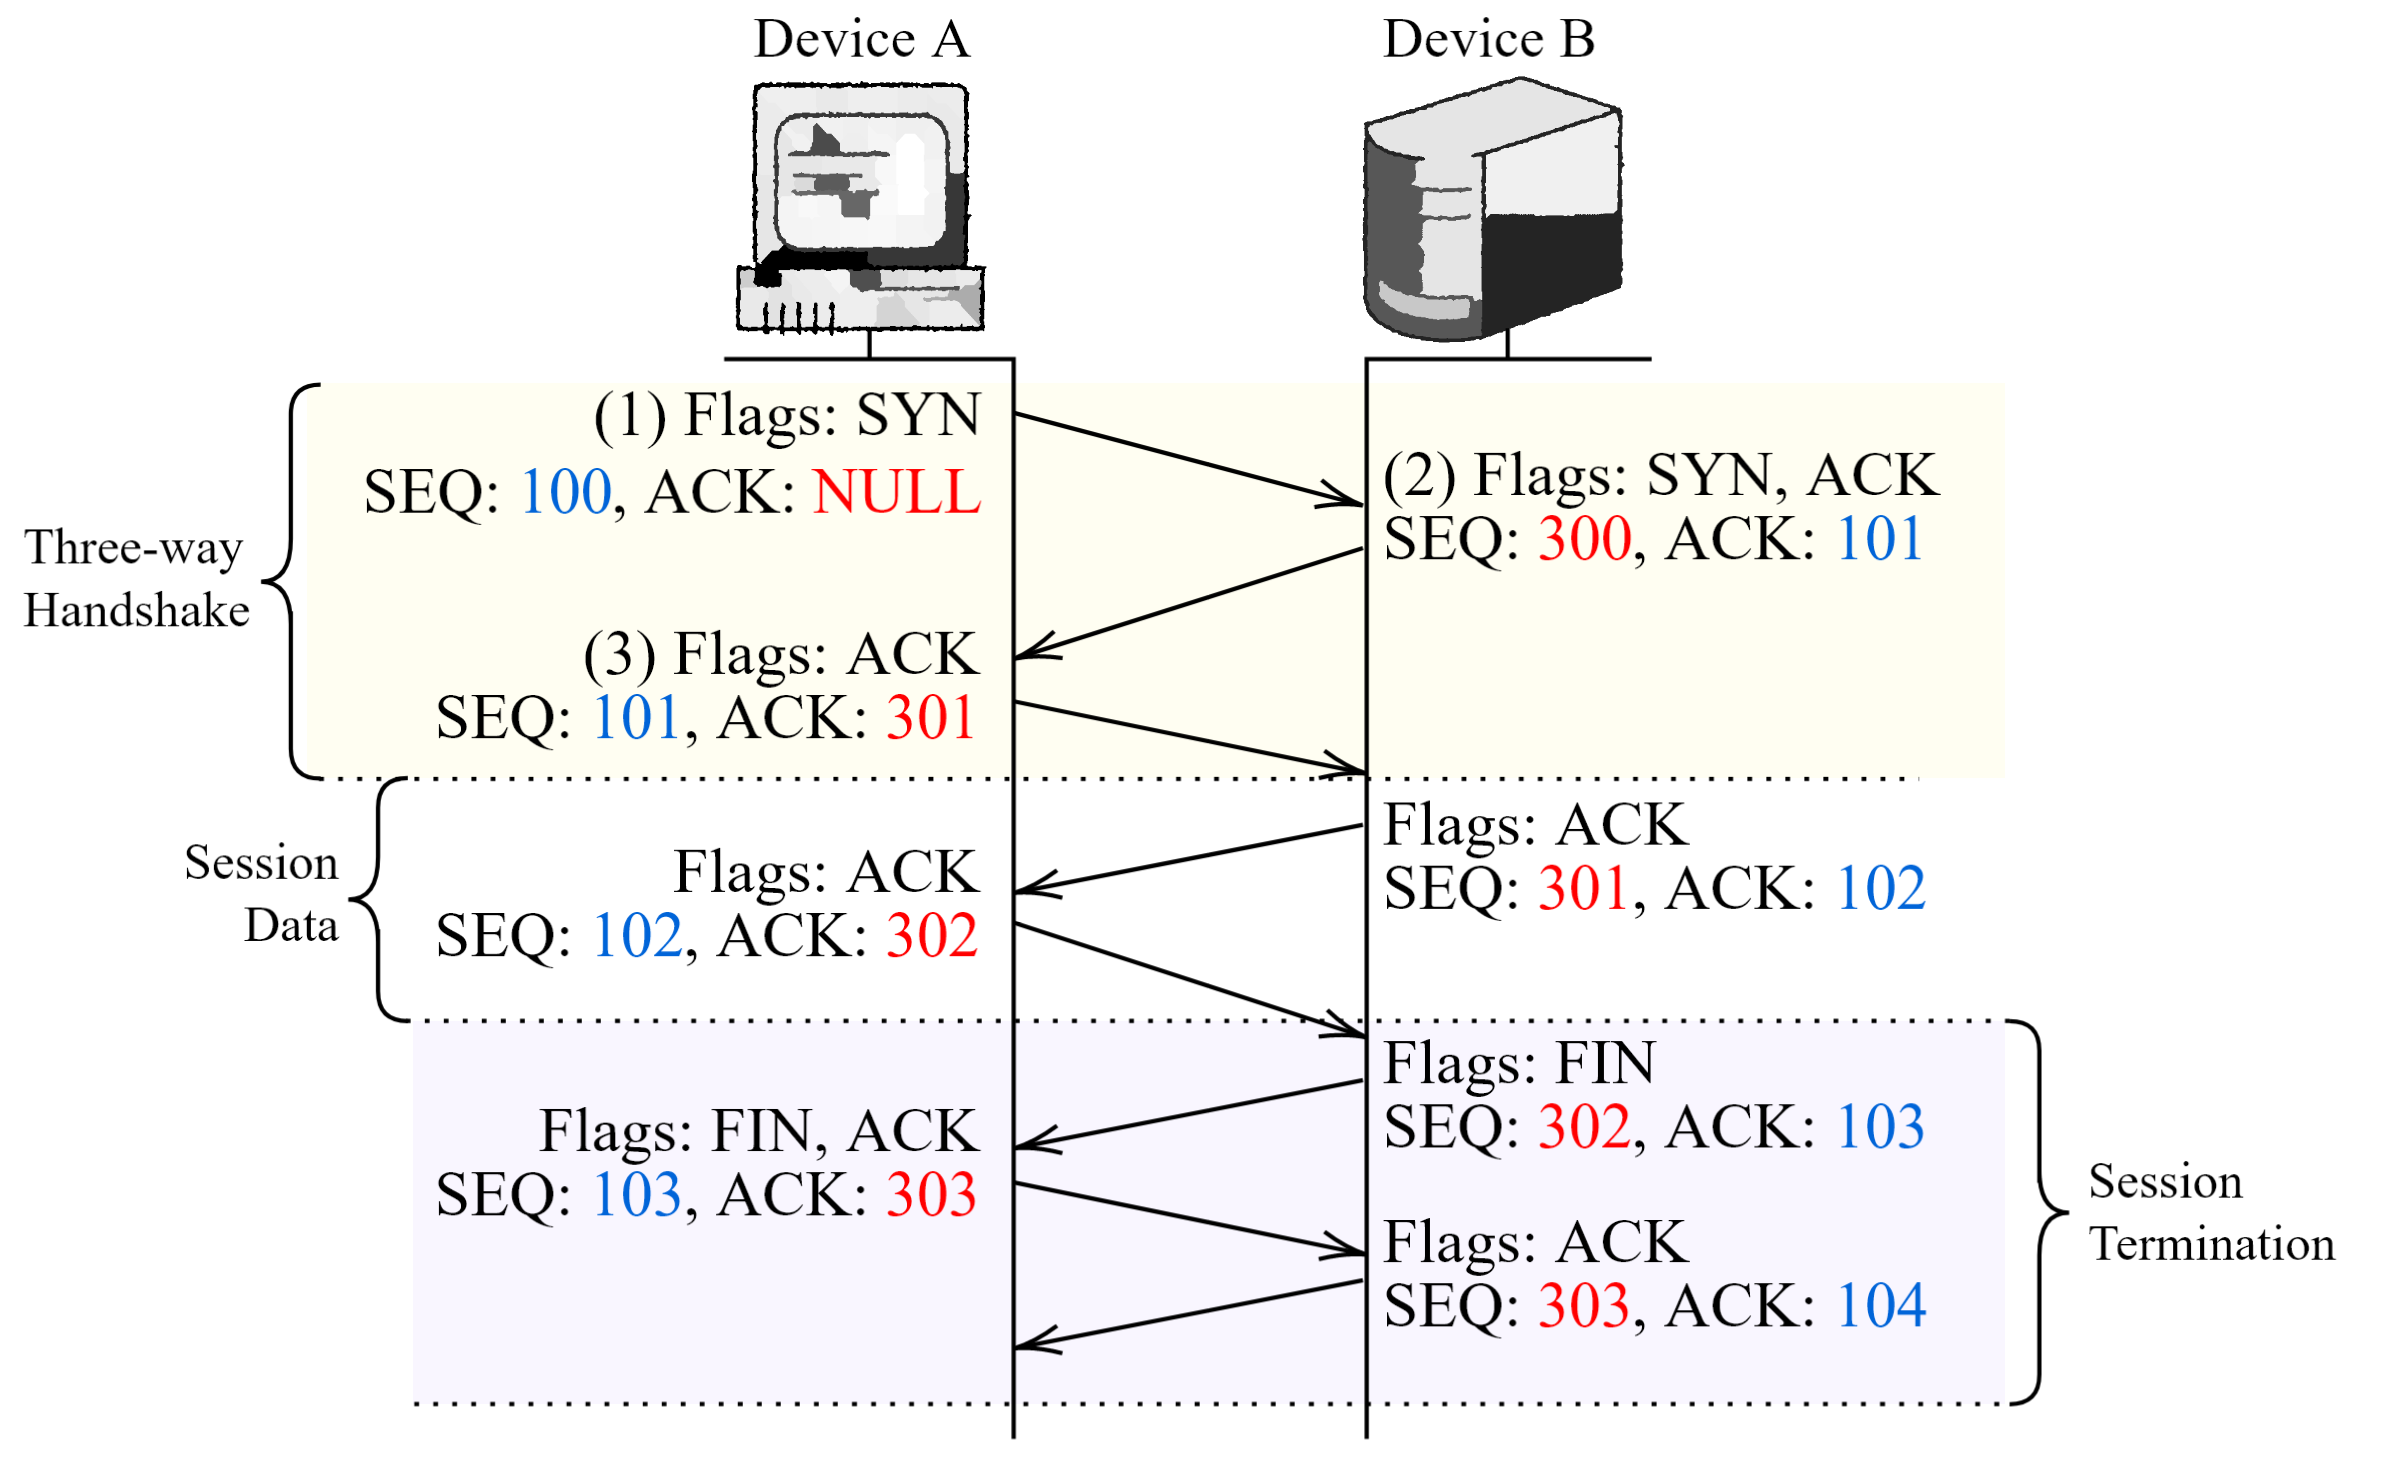
\includegraphics[width=0.9\textwidth]{Sections/network/synack.png}
    \caption{SYN-ACK Handshake, showing Sequence (SEQ) and Acknowledgment (ACK) Numbers.}
    \label{fig:tcp_options}
\end{figure}

\newpage

\begin{Def}[TCP Windows]

    The \textbf{TCP Window} is a flow control mechanism that determines how much data can be sent before receiving an acknowledgment from the receiver. 
    The size of the window is specified by the \textbf{Window Size} field in the TCP header and can dynamically adjust during the connection.\\

    \noindent
    E.g., Consider a window allowance of 10 packets. If the sender is still waiting on an ACK for packet 1 while it has sent out packets 2-10, the window size reduces momentarily
    waiting for the receiver to acknowledge the first packet before sending more. \hfill \cite{rfc793}
    
\end{Def}

\begin{Def}[UDP Header]

    The \textbf{UDP (User Datagram Protocol) Header} is a fixed-size, lightweight header. 
    It consists of only 8 bytes, containing only essential information. \hfill \cite{rfc768}
\end{Def}

\begin{table}[h]
    \centering
    \resizebox{1\textwidth}{!}{
    \begin{tabular}{|l|c|p{7cm}|}
    \hline
    \textbf{Field}                & \textbf{Size (bits)} & \textbf{Description} \\ \hline
    Source Port                  & 16                  & Identifies the sending application. This field is optional and may be set to zero if not used. \\ \hline
    Destination Port             & 16                  & Identifies the receiving application. \\ \hline
    Length                       & 16                  & Specifies the total length of the UDP packet, including the header and payload, in bytes. \\ \hline
    Checksum                     & 16                  & Provides basic error-checking for the header and payload. If not used, it can be set to zero. \\ \hline
    \end{tabular}
    }
    \caption{Fields of the UDP Header}
    \label{tab:udp-header}
\end{table}    

\begin{figure}[h!]
    \hspace{-2em}
    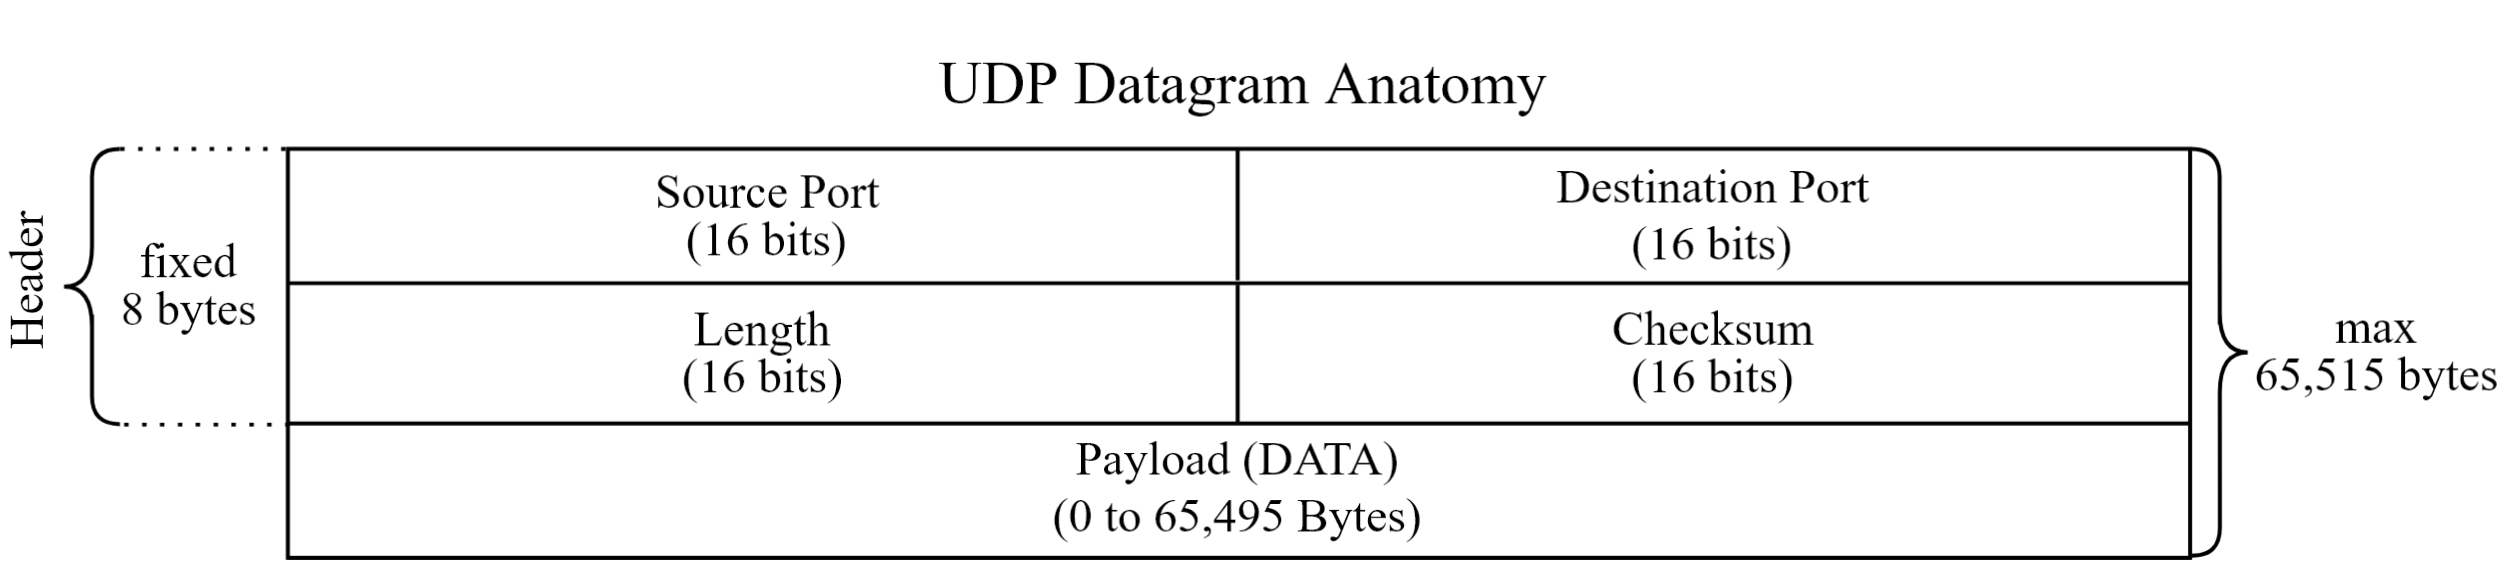
\includegraphics[width=1.1\textwidth]{Sections/network/udp.png}
    \caption{UDP Header}
    \label{fig:udp_header}
\end{figure}

\newpage
\begin{Def}[IPv4 Packet Header]

    An \textbf{IPv4 packet header} as outline in RFC\#791, contains essential information for routing and delivering data across networks. 
    The header consists of several fields, each serving a specific purpose. 
    Eg., [IP Header (20–60 bytes), Transport Header, Payload]. in a stream of bits. \hfill \cite{rfc791}
\end{Def}
\begin{figure}[h!]
    \centering
    \resizebox{1\textwidth}{!}{
        \begin{tabular}{|l|c|p{7cm}|}
        \hline
        \textbf{Field} & \textbf{Size (bits)} & \textbf{Description} \\ \hline
        Version & 4 & Specifies the IP version; for IPv4, this value is 4. \\ \hline
        Internet Header Length (IHL) & 4 & Indicates the header length in 32-bit words; minimum value is 5 (20 bytes). \\ \hline
        Type of Service (ToS) & 8 & Defines packet priority and request for specific handling, such as low delay or high throughput. \\ \hline
        Total Length & 16 & Total size of the packet (header and data) in bytes; minimum is 20 bytes, maximum is 65,535 bytes. \\ \hline
        Identification & 16 & Unique identifier for fragmenting and reassembling packets. \\ \hline
        Flags & 3 & Control flags for fragmentation: Reserved (1 bit), Don't Fragment (1 bit), More Fragments (1 bit). \\ \hline
        Fragment Offset & 13 & Specifies the position of this fragment in the original packet; measured in 8-byte blocks. \\ \hline
        Time to Live (TTL) & 8 & Limits the packet's lifespan; decremented by each router, and discarded when reaching zero to prevent infinite loops. \\ \hline
        Protocol & 8 & Indicates the encapsulated protocol (e.g., 6 for TCP, 17 for UDP). \\ \hline
        Header Checksum & 16 & Error-checking of the header; recalculated at each hop. \\ \hline
        Source Address & 32 & IP address of the sender. \\ \hline
        Destination Address & 32 & IP address of the receiver. \\ \hline
        Options & 0-320 & Optional settings for control, routing, or security; length varies and is not commonly used. \\ \hline
        Padding & Variable & Added to ensure the header length is a multiple of 32 bits. \\ \hline
        \end{tabular}
    }
    \caption{IPv4 Packet Header Fields}
    \label{tab:ipv4-header}
\end{figure}

\newpage 


\begin{figure}[h!]
    \hspace{-2.5em}
    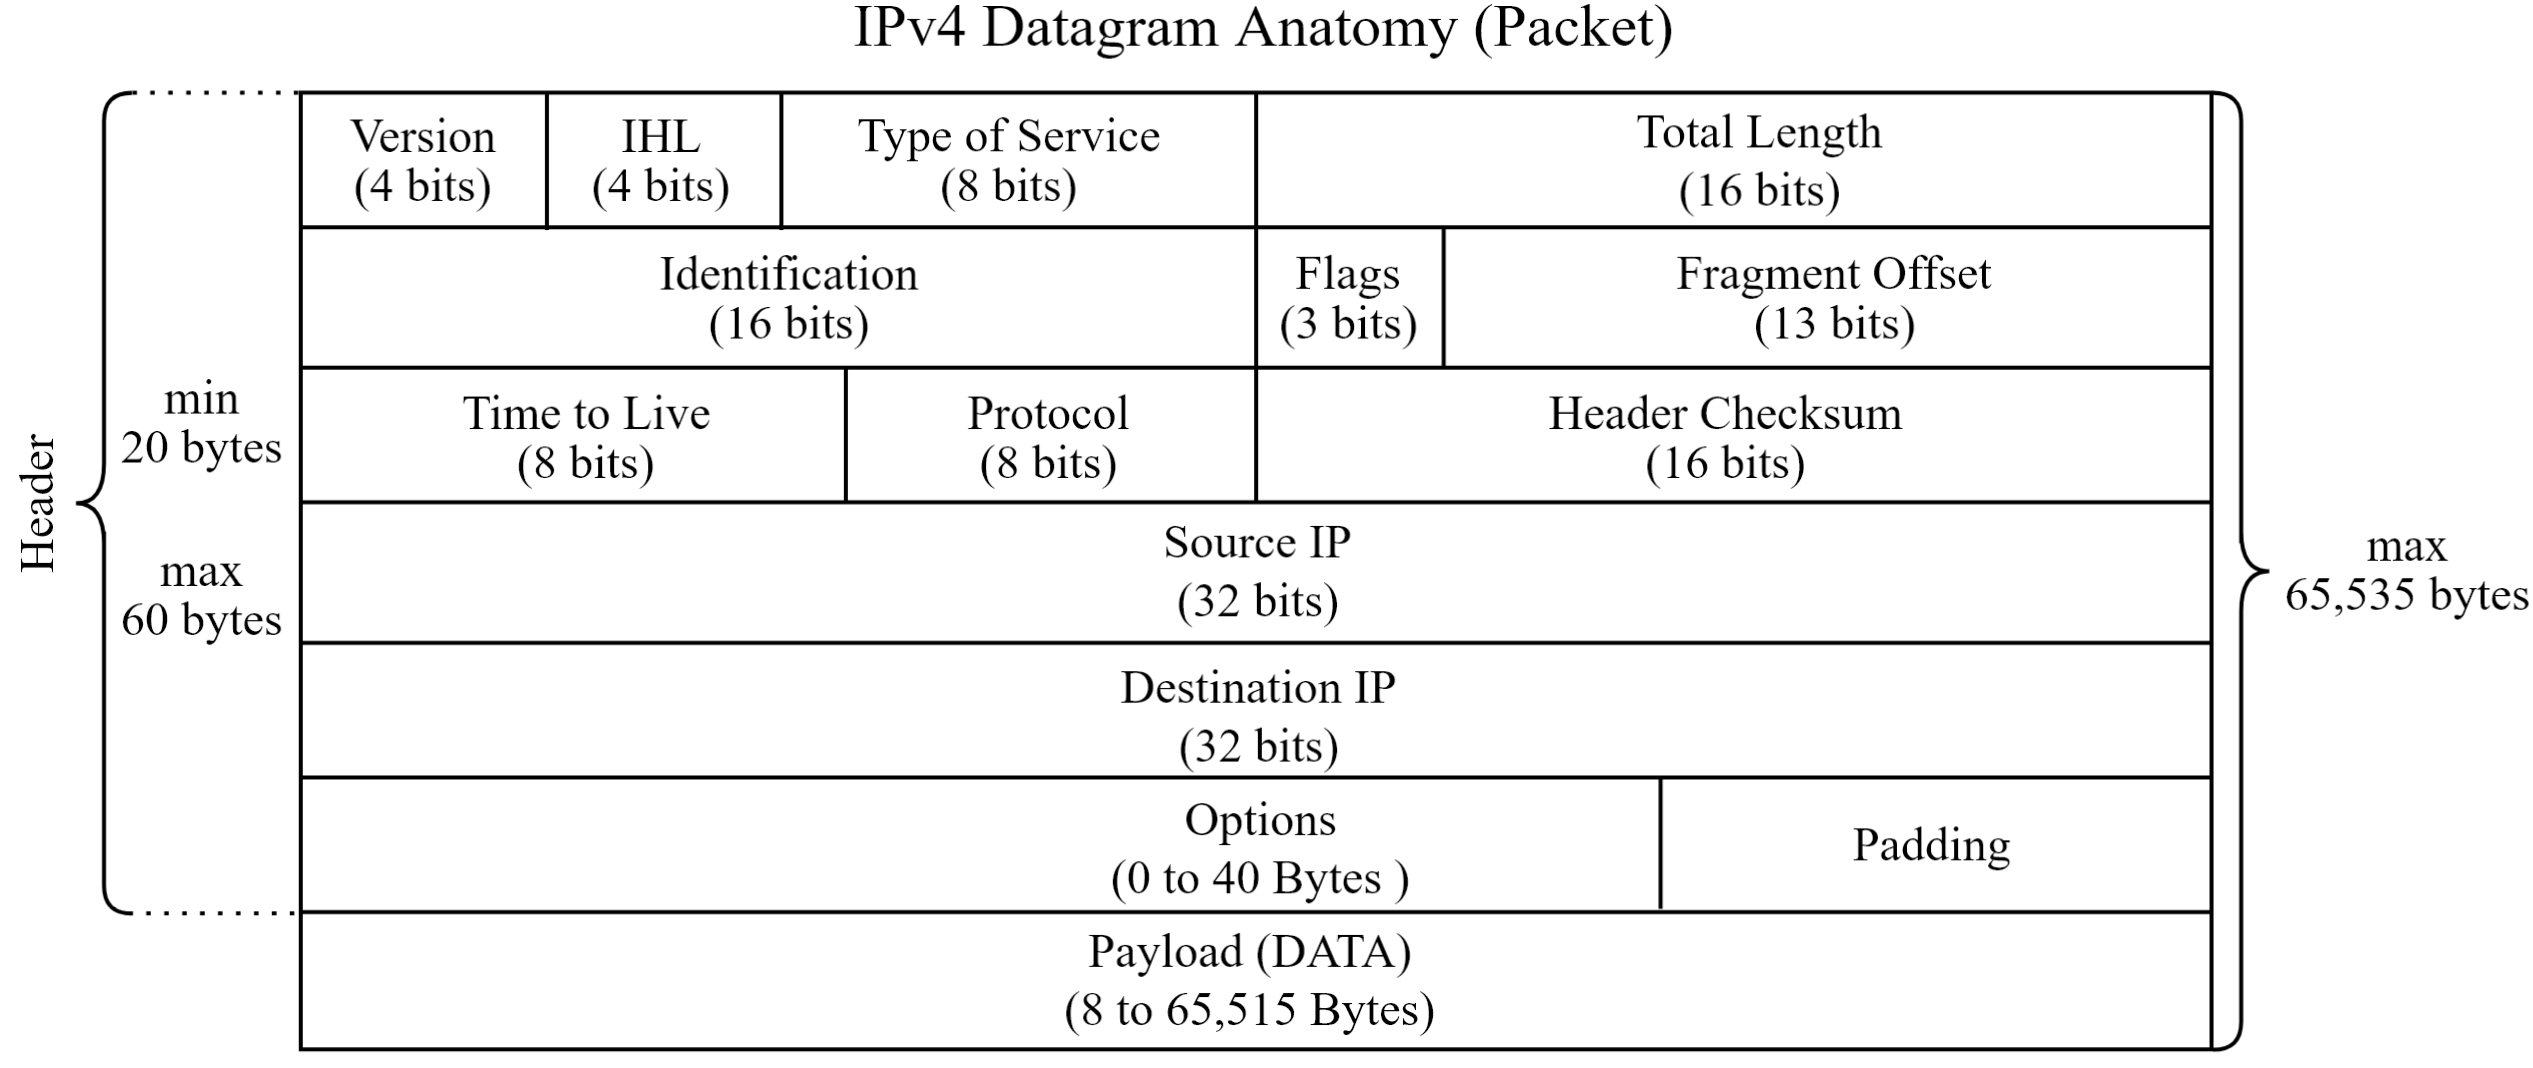
\includegraphics[width=1.1\textwidth]{Sections/network/datagram.png}
    \caption{IPv4 Packet Header.}
    \label{fig:ipv4_header}
\end{figure}

\noindent
Payload is possibly 8-65,515 bytes, because of UDP's 8-byte header. Normally the size is variable, and much more in 
the ball park of 1,500 bytes.
\begin{Def}[IPv4 Flags]

    
    \textbf{Reserved (Bit 0)}: Reserved for future use, must be set to \texttt{0}.\\
    \textbf{Don't Fragment (DF, Bit 1)}: \texttt{0}: Fragmenting allowed. 
    \texttt{1}: Fragmented prohibited; if required, the packet is discarded, and an ICMP error (next definition) is sent to the sender.\\
    \textbf{More Fragments (MF, Bit 2)}: \texttt{0}: Last fragment. \texttt{1}: More fragments are expected. \hfill \cite{rfc791}
    
\end{Def}


\begin{Def}[Internet Control Message Protocol (ICMP)]

    \textbf{Internet Control Message Protocol (ICMP)} is a supporting protocol used by network devices to communicate error messages and operational information. To name a few:
    \begin{itemize}
        \item \textbf{Destination Unreachable}: Indicates that a packet could not reach its destination.
        \item \textbf{Time Exceeded}: Signals that the packet's \textbf{Time to Live (TTL)} has expired.
        \item \textbf{Fragmentation Needed}: Informs the sender the packet is too large without fragmenting.
        \item \textbf{Echo Request and Reply (Ping)}: Tests connectivity between devices. \hfill \cite{rfc792}
    \end{itemize}
    \noindent
    For full specifications visit: \href{https://www.iana.org/assignments/icmp-parameters/icmp-parameters.xhtml}{ICMP Parameters}. Note viewing their reference RFCs may be more informative.
\end{Def}

    
\newpage

\begin{Def}[IPv4 Options]

    The \textbf{IPv4 Options} field is an optional. Every options occupies 1 byte regardless do data\\
    \hfill (var = variable, `-' = none).
    
    \textbf{Common IPv4 Options (class, number, data length (bytes))}:
    \begin{itemize}
        \item \textbf{End of Option List (0, 0, -)}: Marks the end of the options field.
        \item \textbf{No Operation (0, 1, -)}: Used for padding.
        \item \textbf{Security (0, 2, 11)}: Includes security and compartmentalization details.
        \item \textbf{Loose Source Routing (0, 3, var)}: Specifies a loose route for pathing.
        \item \textbf{Internet Timestamp (2, 4, var)}: Records timestamps at each hop.
        \item \textbf{Strict Source Routing (0, 9, var)}: Specifies an exact route for pathing.
        \item \textbf{Record Route (0, 7, var)}: Records the route taken by the datagram.
        \item \textbf{Stream ID (0, 8, 4)}: Identifies the stream of communication.
    \end{itemize}

    \noindent
    \textbf{Classes:} \textbf{0}: Control. \textbf{1}: Reserved for future use. \textbf{2}: Debugging and Measurement.\\
    \textbf{3}: Reserved for future use. \hfill \cite{rfc791}
\end{Def}

\noindent
\underline{\textbf{QUIC Headers} will be introduced later,} as it incorporates uncovered content. The following solution was implemented to address the exhaustion of IPv4 addresses:
\begin{Def}[Private and Public IP Addresses]

    IP addresses are classified as \textbf{private} or \textbf{public} based on their scope and accessibility:
    \begin{itemize}
        \item \textbf{Private IP Addresses}: Reserved for use within private networks (e.g., home or corporate networks). These addresses cannot communicate directly over the internet and include ranges like:
            \begin{itemize}
                \item[>] \(10.0.0.0 - 10.255.255.255\)
                \item[>] \(172.16.0.0 - 172.31.255.255\)
                \item[>] \(192.168.0.0 - 192.168.255.255\)
            \end{itemize}
        \item \textbf{Public IP Addresses}: Globally unique addresses assigned by the Internet Assigned Numbers Authority (IANA) for communication over the internet.
    \end{itemize}

    \noindent
    Devices on a private network can communicate internally using private IPs, while a public IP is needed to access external networks like the internet. Communication between these address types is facilitated by \textbf{Network Address Translation (NAT)}.
    \hfill \cite{rfc1918}
\end{Def}


\begin{Def}[Network Address Translation (NAT)]

    \textbf{Network Address Translation (NAT)} is a networking technique that translates private IP addresses within a local network to a public IP address for communication over external networks, such as the internet.
    NAT modifies the source IP address in outbound packets and reverses the process for inbound packets, ensuring data is correctly routed to devices within the private network.

    NAT enables multiple devices to share a single public IP address,
    facilitating efficient communication while keeping private IP addresses hidden from external networks.  \hfill \cite{rfc1918}\cite{rfc2663}   
\end{Def}

\vspace{-1em}
\begin{Def}[Dynamic \& Static NATs and PATs]

    When a device crosses a router into an external network, the router replaces parts of the packet with a public translation.
    There are \textbf{NATs} and \textbf{Port Address Translations (PATs)}:

    \begin{itemize}
        \item \textbf{NAT}: Only translates the IP address, leaving the port unchanged.
        \item \textbf{PAT}: Translates both the IP address and port number (rarely, only the port).
    \end{itemize}

    \noindent
    There are two types of configurations for NAT and PAT:
    \begin{itemize}
        \item \textbf{Static:} The administrator explicitly defines the translations of IP addresses and ports.
        \item \textbf{Dynamic:} The administrator defines a pool of public IP addresses and ports, allowing the router to assign them dynamically.
    \end{itemize}

    \noindent
    PATs are referred to in RFC\#2663 as \textbf{Network Address Port Translation (NAPT)}. This overall process is also known as \textbf{Overloading} or 
    \textbf{IP Masquerading}. \hfill \cite{rfc2663}

\end{Def}

\vspace{-1.5em}

\begin{figure}[h!]
    \hspace{-1em}
    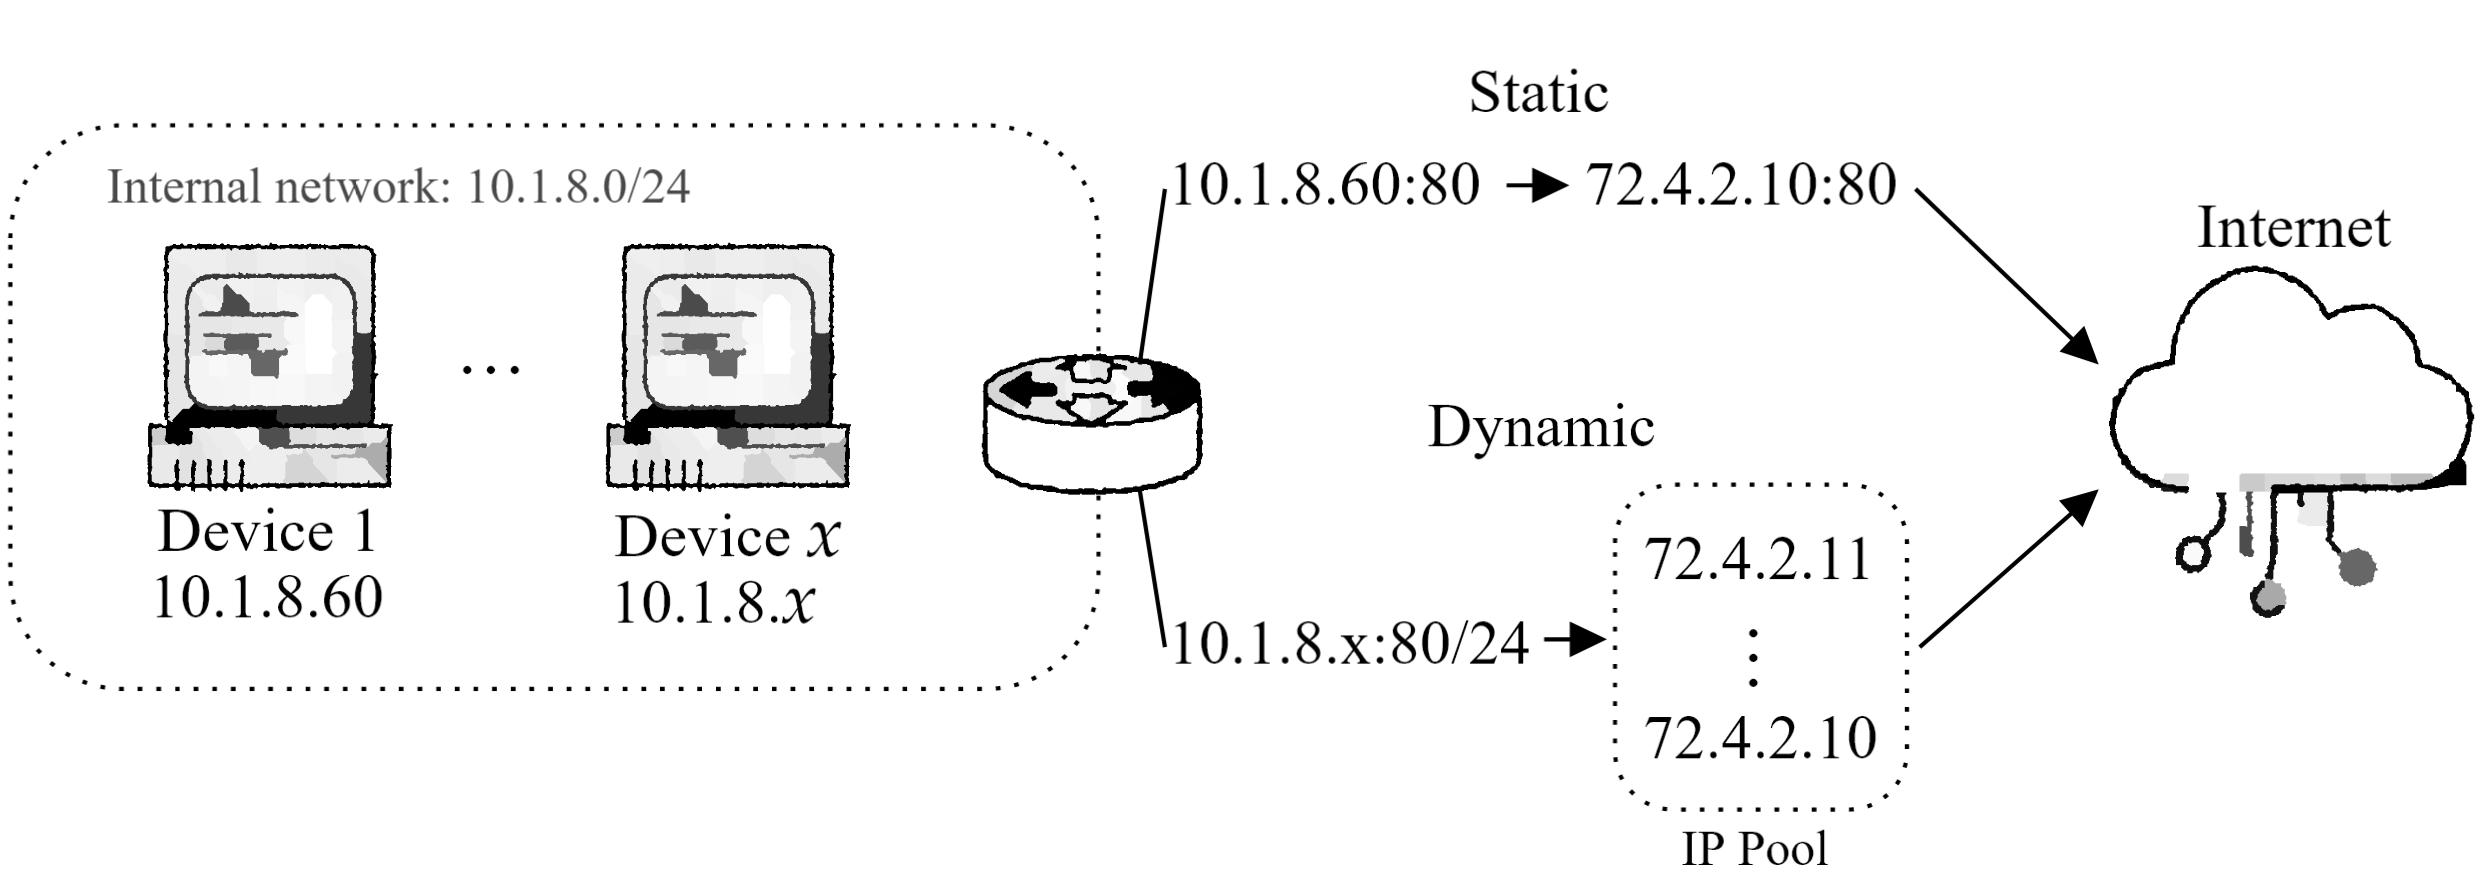
\includegraphics[width=1\textwidth]{Sections/network/nat.png}
    \caption{Static and Dynamic NATs from an internal network to the internet.}
    \label{fig:nat}
\end{figure}

\noindent
Incoming traffic will reverse the process, translating the public IP back into its private mapping. In many 
cases, an administrator would be an ISP, who distributes public IPs to clients.

\newpage 

\begin{Def}[Regional Internet Registries (RIRs)]

    \textbf{Regional Internet Registries (RIRs)} are non-profit organizations responsible for the allocation, distribution, and management of Internet number resources, including \textbf{IPv4 and IPv6 addresses} and \textbf{Autonomous System Numbers (ASNs)}, within specific geographic regions.
    
    \noindent
    \textbf{Key Functions of RIRs:}
    \begin{itemize}
        \item \textbf{Database Management}: Maintain public records documenting the allocation and assignment of Internet number resources.
        \item \textbf{Policy Development}: Facilitate community-driven processes for creating policies on resource management.
    \end{itemize}

    \noindent
    \textbf{The Five RIRs and Their Regions:}
    \begin{itemize}
        \item \textbf{ARIN}: North America, Canada, parts of the Caribbean.
        \item \textbf{RIPE NCC}: Europe, the Middle East, and Central Asia.
        \item \textbf{APNIC}: Asia and the Pacific region.
        \item \textbf{LACNIC}: Latin America and parts of the Caribbean.
        \item \textbf{AFRINIC}: Africa and the Indian Ocean region.
    \end{itemize}
    
    \hfill \cite{rir_overview}
\end{Def}


\begin{Def}[Carrier-Grade NAT (CGNAT/NAT444)]

    \textbf{Carrier-Grade NAT (CGNAT)}, also known as \textbf{NAT444}, is a network translation mechanism used by Internet Service Providers (ISPs) to address IPv4 address exhaustion. It refers to three sets of IPv4 addresses:
    \begin{itemize}
        \item \textbf{Customer Private}: IPv4 addresses within the customer's local network.
        \item \textbf{ISP Private}: IPv4 addresses used internally within the ISP's network.
        \item \textbf{Public Internet}: IPv4 addresses used for external communication.
    \end{itemize}
    
    Network Address Translation occurs in two stages:
    \begin{itemize}
        \item \textbf{Customer Private → ISP Private}: Translation by the customer's router---\textbf{Customer Premises Equipment (CPE)}.
        \item \textbf{ISP Private → Public Internet}: Translation by the ISP's CGNAT device.
    \end{itemize}

    \hfill \cite{rfc2663}\cite{rbfs_cgnat}
    
\end{Def}
    
\newpage

\begin{figure}[h!]
    \hspace{-2.5em}
    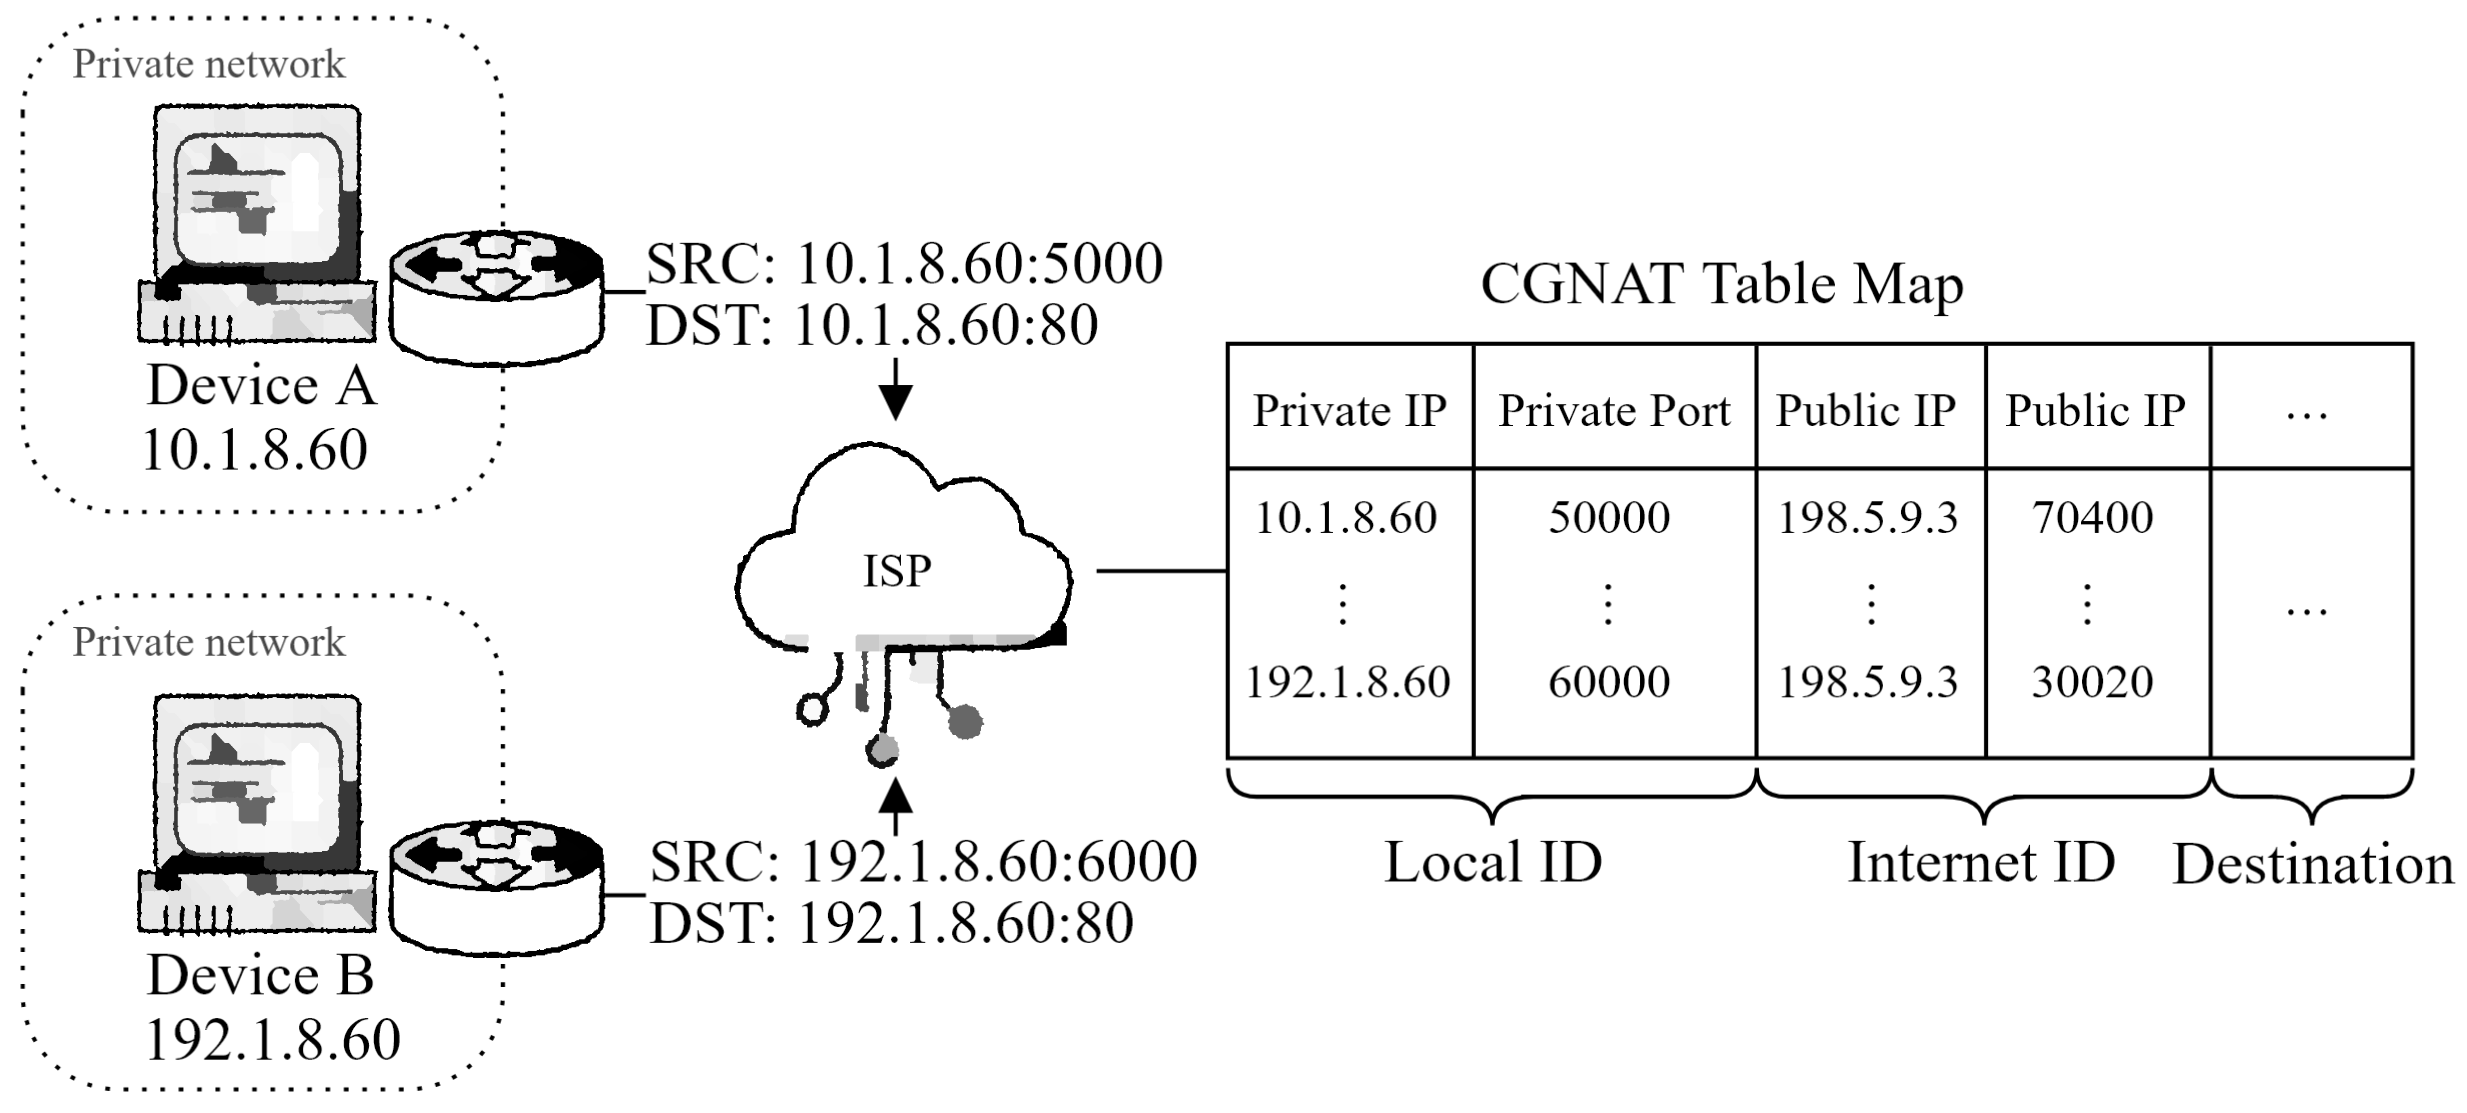
\includegraphics[width=1.1\textwidth]{Sections/network/cgnat.png}
    \caption{Carrier-Grade NAT (CGNAT) Translation Process}
    \label{fig:cgnat}
\end{figure}

\begin{Def}[DNS Servers]

    \textbf{Domain Name System (DNS) Servers} are specialized servers responsible for translating human-readable domain names (e.g., \texttt{example.com}) into machine-readable IP addresses (e.g., \texttt{192.0.2.1}),
    a process known as a \textbf{DNS Lookup}. Retrieving a website involves:
    \begin{itemize}
        \item Querying DNS servers to resolve a domain name into its corresponding IP address.
        \item Traversing a hierarchical network of DNS servers: starting from \textbf{root servers}, through \textbf{Top-Level Domain (TLD) servers} (e.g., \texttt{.com}), to the \textbf{authoritative DNS server} for the domain.
    \end{itemize}
    
    \noindent
    \textbf{Control and Operation}:
    \begin{itemize}
        \item \textbf{Root DNS Servers} are managed by independent organizations under the coordination of the \textbf{Internet Corporation for Assigned Names and Numbers (ICANN)}.
        \item \textbf{TLD DNS Servers} manage domains under specific extensions like \texttt{.com}, \texttt{.org}, and country-specific domains like \texttt{.uk}.
        \item \textbf{Authoritative DNS Servers} are controlled by entities that manage specific domain names, including private companies, governments, or educational institutions.
    \end{itemize}
    
    \noindent
    \textbf{Caching}: Devices (e.g., computers, routers) and services (e.g., ISPs) may store previously resolved domain names in a \textbf{DNS cache}, reducing the need for repeated lookups and improving connection speed. \hfill \cite{rfc1034}
    
    
\end{Def}

\newpage

\begin{figure}[h!]
    \hspace{-2.5em}
    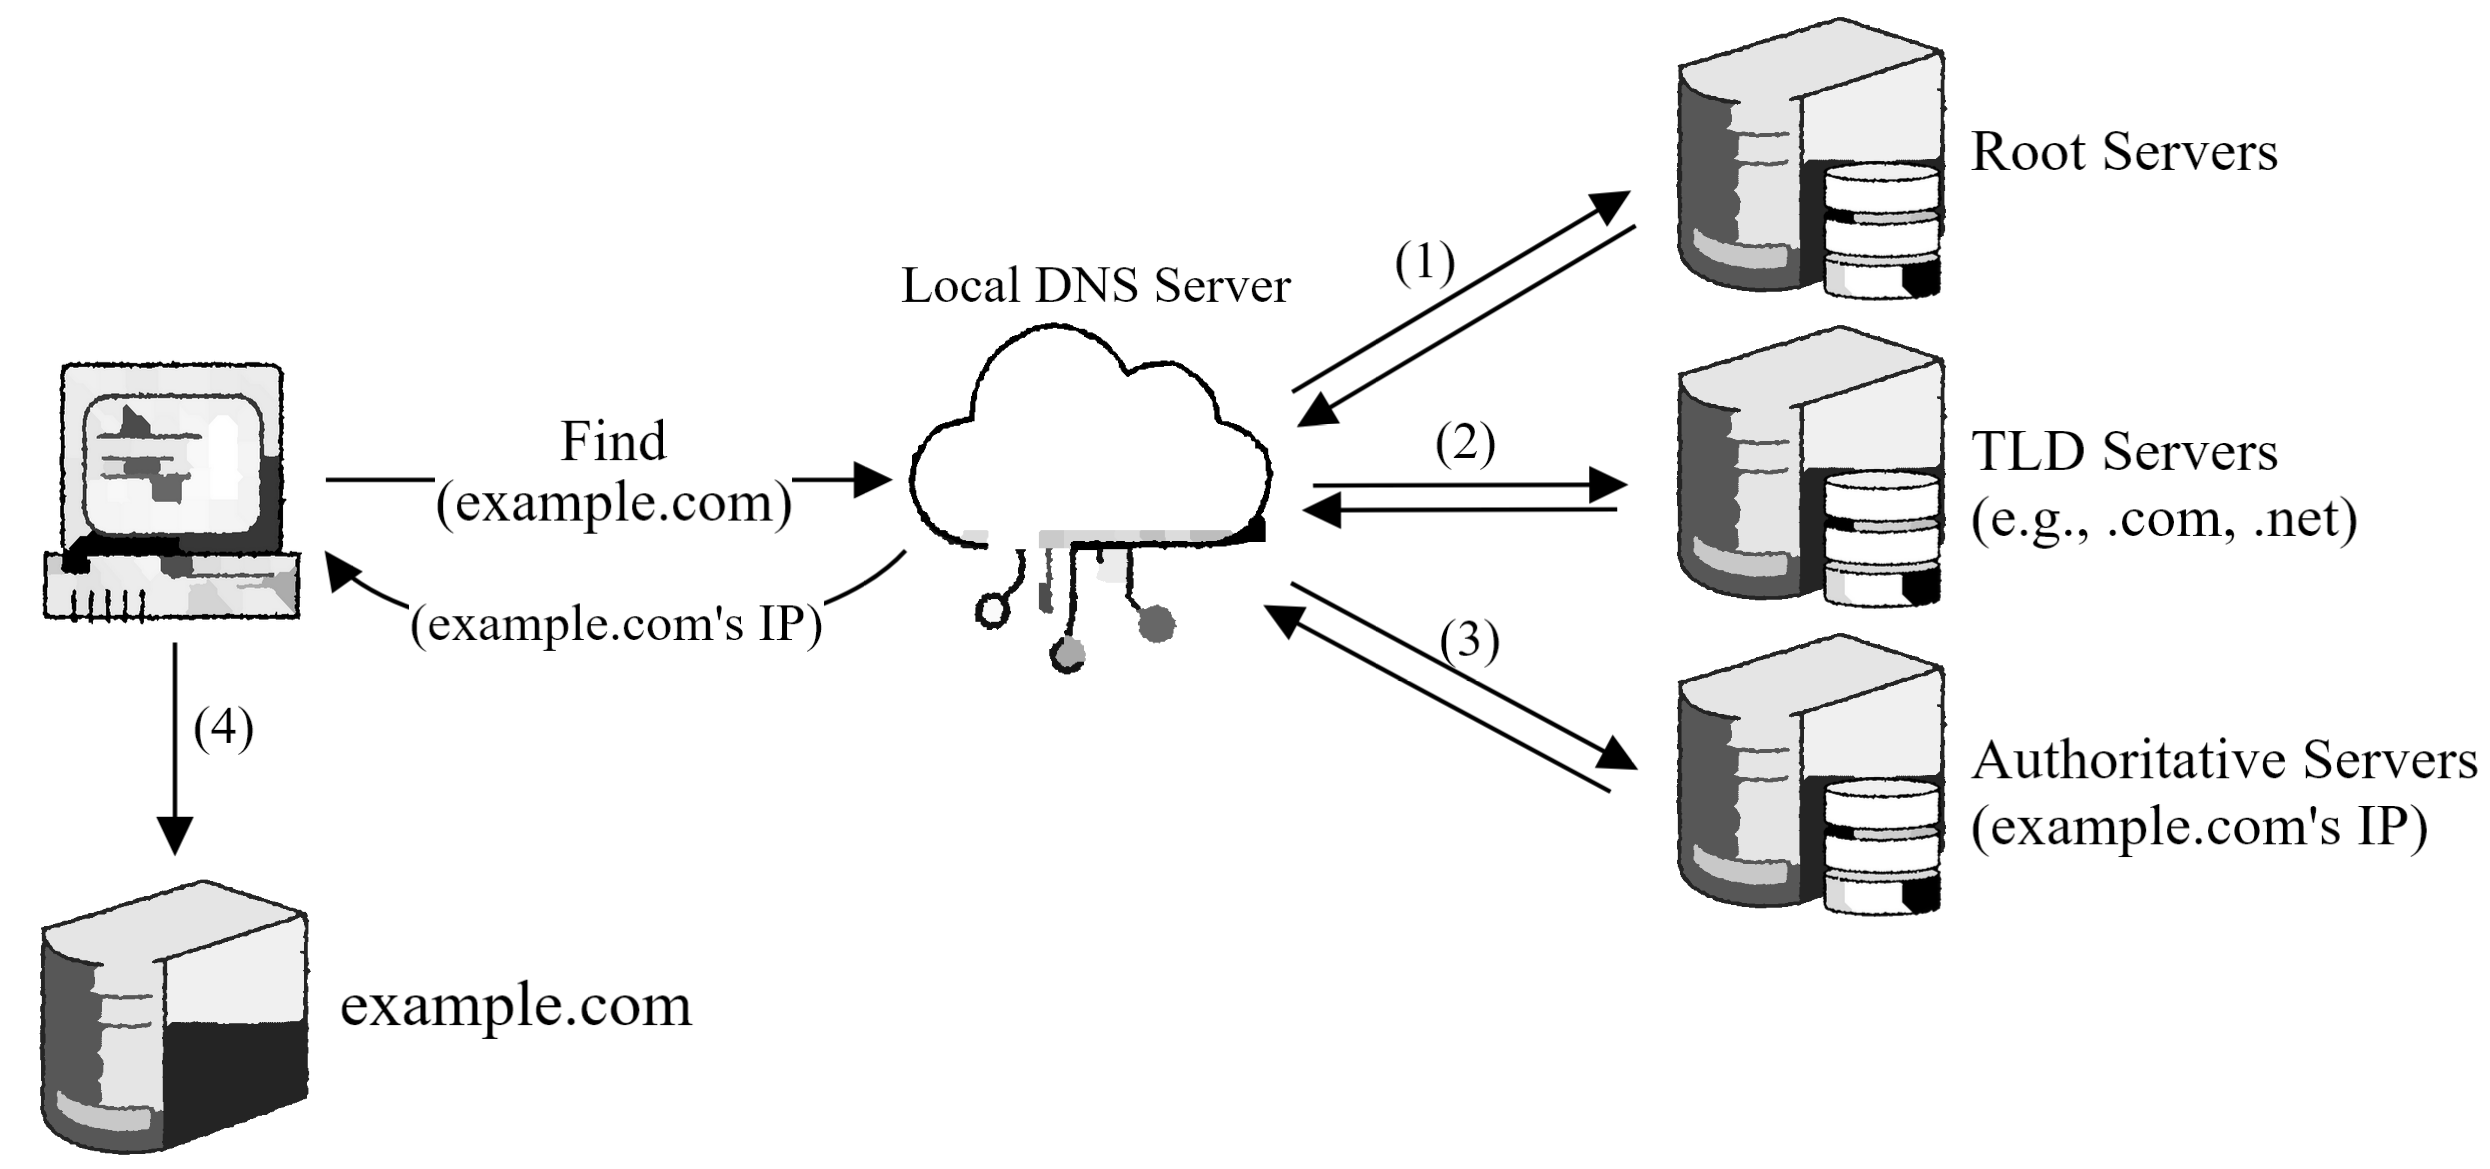
\includegraphics[width=1.1\textwidth]{Sections/network/dns.png}
    \caption{DNS Lookup Process: (1). Query root server for (\texttt{.com}), (2). Query TLD for (\texttt{example.com}), (3). Query Authority for (\texttt{example.com's IP}).}
    \label{fig:dns}
\end{figure}

\begin{Def}[DNS Hierarchy: Root, TLD, and Authoritative Servers]

    \begin{itemize}
        \item \textbf{Root Servers}:
        Only provide references to the appropriate \textbf{TLD servers} based on the queried domain extension (e.g., \texttt{.com}, \texttt{.org}).
        \begin{itemize}
            \item Operated by organizations like VeriSign, USC, and ICANN.
            \item Example: The \texttt{A} Root Server is managed by VeriSign.
            \item View the full list at: \url{https://root-servers.org/}.
        \end{itemize}
    
        \item \textbf{TLD Servers}:
        Manages \textbf{Top-Level Domains (TLDs)} such as \texttt{.com}, \texttt{.org}, and \texttt{.uk}. They direct queries to the \textbf{authoritative servers} for the requested domain.
        \begin{itemize}
            \item Example: VeriSign manages TLD servers for \texttt{.com} and \texttt{.net}.
            \item Often operated by private companies or regional internet registries.
        \end{itemize}
    
        \item \textbf{Authoritative Servers}:
        These servers store DNS records for specific domain names, responding with the IP address of the queried domain.
        \begin{itemize}
            \item Example: A hosting provider like AWS or Google Cloud might manage the authoritative server for \texttt{example.com}.
            \item Businesses, ISPs, or hosting services typically operate these servers.
        \end{itemize}
    \end{itemize}
    
    \hfill \cite{iana_root_servers}\cite{cloudflare_dns_server_types}
\end{Def}

\newpage

\begin{Def}[HTTP Messages]

    When communicating with a web server, a client establishes an \textbf{HTTP session} to exchange data.
    The client sends an \textbf{HTTP request} to the server, which processes the request and responds with an \textbf{HTTP response}.
    The HTTP header and Response consists of:
    \begin{enumerate}
        \item \textbf{Request Line}: Contains the request method (e.g., GET, POST), URL, and HTTP version.
        \item \textbf{Request Headers}: Include additional information such as DNS and client software.
        \item \textbf{Empty Line}: Separates the header from the body.
        \item \textbf{Request Body}: Contains data sent to the server (e.g., form data). Optional for some requests (e.g., GET). 
    \end{enumerate}

    \noindent
    Messages are sent over \textbf{TCP} or \textbf{UDP} stored in the \textbf{Payload} of the datagram. \hfill \cite{fielding_http_1999}
\end{Def}

\begin{Def}[Uniform Resource Identifier (URI) \& URLs]

    A \textbf{Uniform Resource Identifier (URI)}: a string which identifies resources on the web.\\
    A \textbf{Uniform Resource Locator (URL)} a subset of URI that specifies the resource and its location.
    A \textbf{Uniform Resource Name (URN)} is a URI under a different schema, a unique global 
    identifier of a resource even after it is no longer available (e.g., a book isbn, urn:isbn:0451450523). \hfill \cite{berners_lee_uri_2005}
\end{Def} 

\begin{figure}[h!]
    \hspace{-2.5em}
    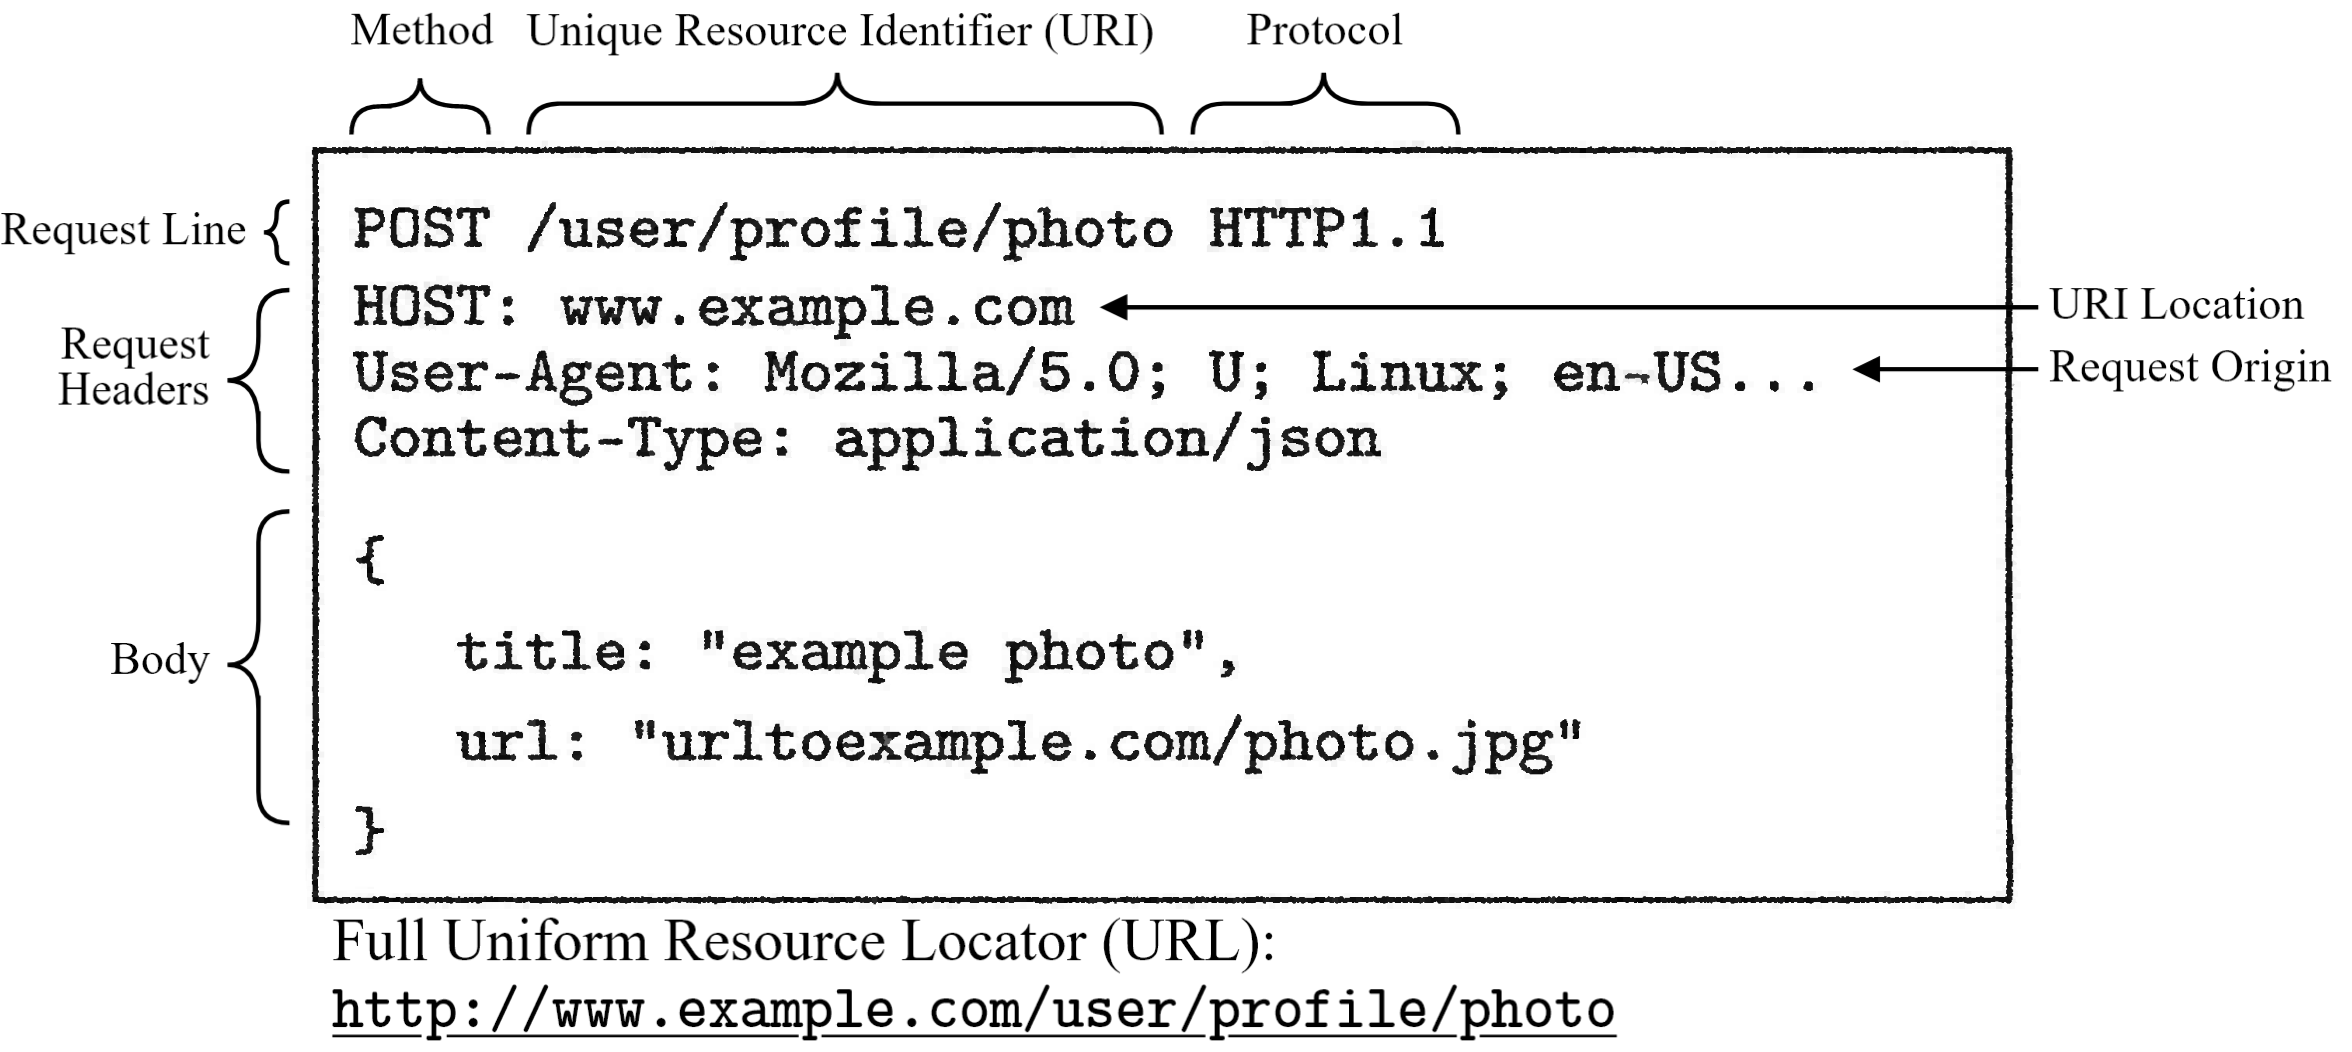
\includegraphics[width=1\textwidth]{Sections/network/httpheader.png}
    \caption{HTTP Request and Response Structure}
    \label{fig:http}
\end{figure}

\newpage

\begin{Def}[Ethernet Frame]
    
    \textbf{Ethernet Frames} at the \textbf{Data Link Layer} (ISO model), encapsulate IP packets for transmission over a local network.
    The specifications for Ethernet, including frame structure and operational parameters, are defined by the \textbf{Institute of Electrical and Electronics Engineers (IEEE)} in the \textbf{IEEE 802.3} standard. \cite{8457469}
\end{Def}
\begin{table}[h!]
    \centering
    \resizebox{1\textwidth}{!}{
    \begin{tabular}{|l|c|p{7cm}|}
    \hline
    \textbf{Field} & \textbf{Size (bytes)} & \textbf{Description} \\ \hline
    \textbf{Preamble} & 7 & A sequence of alternating 1s and 0s (10101010) used for synchronization between the sending and receiving devices. \\ \hline
    \textbf{Start Frame Delimiter (SFD)} & 1 & Indicates the start of the frame; typically has the bit pattern 10101011. \\ \hline
    \textbf{Destination MAC Address} & 6 & The hardware address of the intended recipient. \\ \hline
    \textbf{Source MAC Address} & 6 & The hardware address of the sender. \\ \hline
    \textbf{EtherType/Length} & 2 & Specifies either the protocol type encapsulated in the payload (if $\geq$ 1536) or the length of the payload in bytes (if $\leq$ 1500). \\ \hline
    \textbf{VLAN Tag (optional)} & 4 & Present if IEEE 802.1Q tagging is used; includes Priority Code Point (PCP), Drop Eligible Indicator (DEI), and VLAN Identifier (VID). \\ \hline
    \textbf{Payload} & 46--1500 & The encapsulated data from higher network layers. If the payload is less than 46 bytes, padding is added to meet the minimum frame size requirement. \\ \hline
    \textbf{Frame Check Sequence (FCS)} & 4 & A cyclic redundancy check (CRC) value used to detect errors in the transmitted frame. \\ \hline
    \end{tabular}
    }
    \caption{Structure of an Ethernet Frame}
\end{table}

\begin{figure}[h!]
    \hspace{-2.5em}
    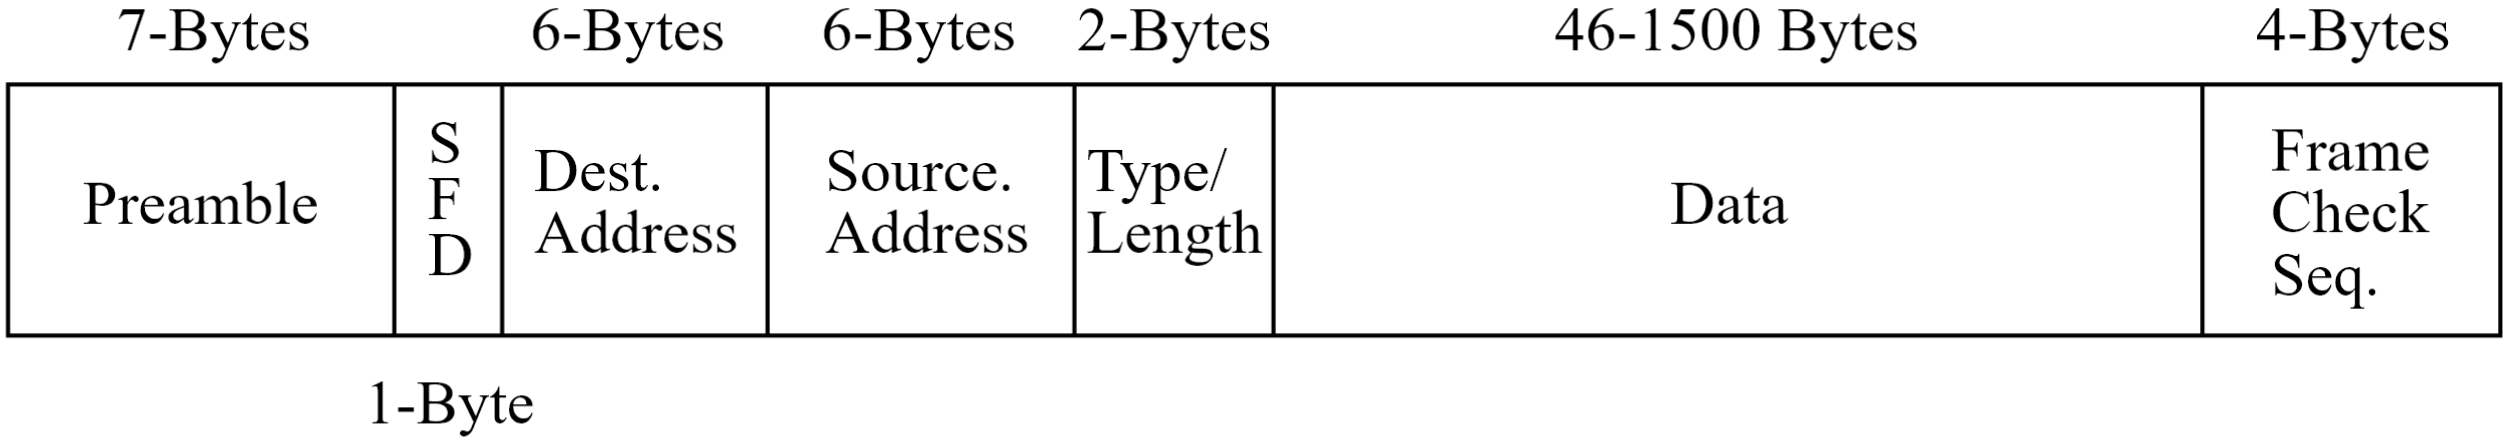
\includegraphics[width=1.1\textwidth]{Sections/network/ethframe.png}
    \caption{Ethernet Frame Structure}
    \label{fig:ethernet}
\end{figure}

\newpage



\begin{theo}[Establishing a Website Connection]

    \begin{enumerate}
        \item \textbf{Application Layer (DNS Request)}:
        The browser initiates a DNS query to resolve the website's domain name (e.g., \texttt{example.com}) into an IP address. The DNS query traverses:
        \begin{itemize}
            \item \textbf{Root DNS Server}$\rightarrow$\textbf{TLD Server}$\rightarrow$\textbf{Authoritative DNS Server}.\\
            (e.g., \texttt{.com}$\rightarrow$\texttt{example.com}$\rightarrow$\texttt{example.com's IP}).
        \end{itemize}
        If the IP address is cached locally or by the ISP, the query resolves faster.
    
        \item \textbf{Transport Layer (Connection Establishment)}:
        After the IP address is resolved, the browser establishes a connection to the server. If using \textbf{TCP}, the connection involves a \textbf{three-way handshake}:
        \begin{itemize}
            \item The browser sends a \textbf{SYN} packet to the server.
            \item The server responds with a \textbf{SYN-ACK} packet.
            \item The browser completes the handshake by sending an \textbf{ACK} packet.
        \end{itemize}
        For protocols like \textbf{UDP}, no handshake occurs, and packets are sent directly without connection establishment.
    
        \item \textbf{Network Layer (Routing)}:
        Packets, regardless of protocol (e.g., TCP, UDP, or ICMP), are encapsulated within IP datagrams and routed to the destination. Routers along the path forward the packets based on the destination IP address in the IP header. The routing process is agnostic to the transport protocol and works universally across all IP-based communication.
    
        \item \textbf{Data Link Layer (Frame Transmission)}:
        If connection is within a local network (e.g., LAN), IP packets incur Ethernet frame encapsulation (or equivalent, depending on the network).
    
        \item \textbf{Physical Layer (Transmission)}:
        Frames are transmitted as electrical signals, light pulses, or radio waves, depending on the physical medium used.
        \textbf{Inter-domain routing protocols}, such as \textbf{OSPF} or \textbf{BGP}, facilitate the transfer of packets through \textbf{AS}es.
        
    
        \item \textbf{Application Layer (HTTP Request)}:
        Once the connection is established, the browser sends an \textbf{HTTP request} to the server via datagram \textbf{Payload}:
        \begin{itemize}
            \item The browser requests the document.
            \item The server responds with the HTML content, which is sent back over the established connection.
        \end{itemize}
    
        \item \textbf{Response and Rendering}:
        The server's response is segmented into TCP packets (if applicable) and reassembled by the browser. The browser processes the HTML and renders the webpage for the user.
    \end{enumerate}

\end{theo}

\newpage
    
\begin{figure}[h!]
    \hspace{-2.5em}
    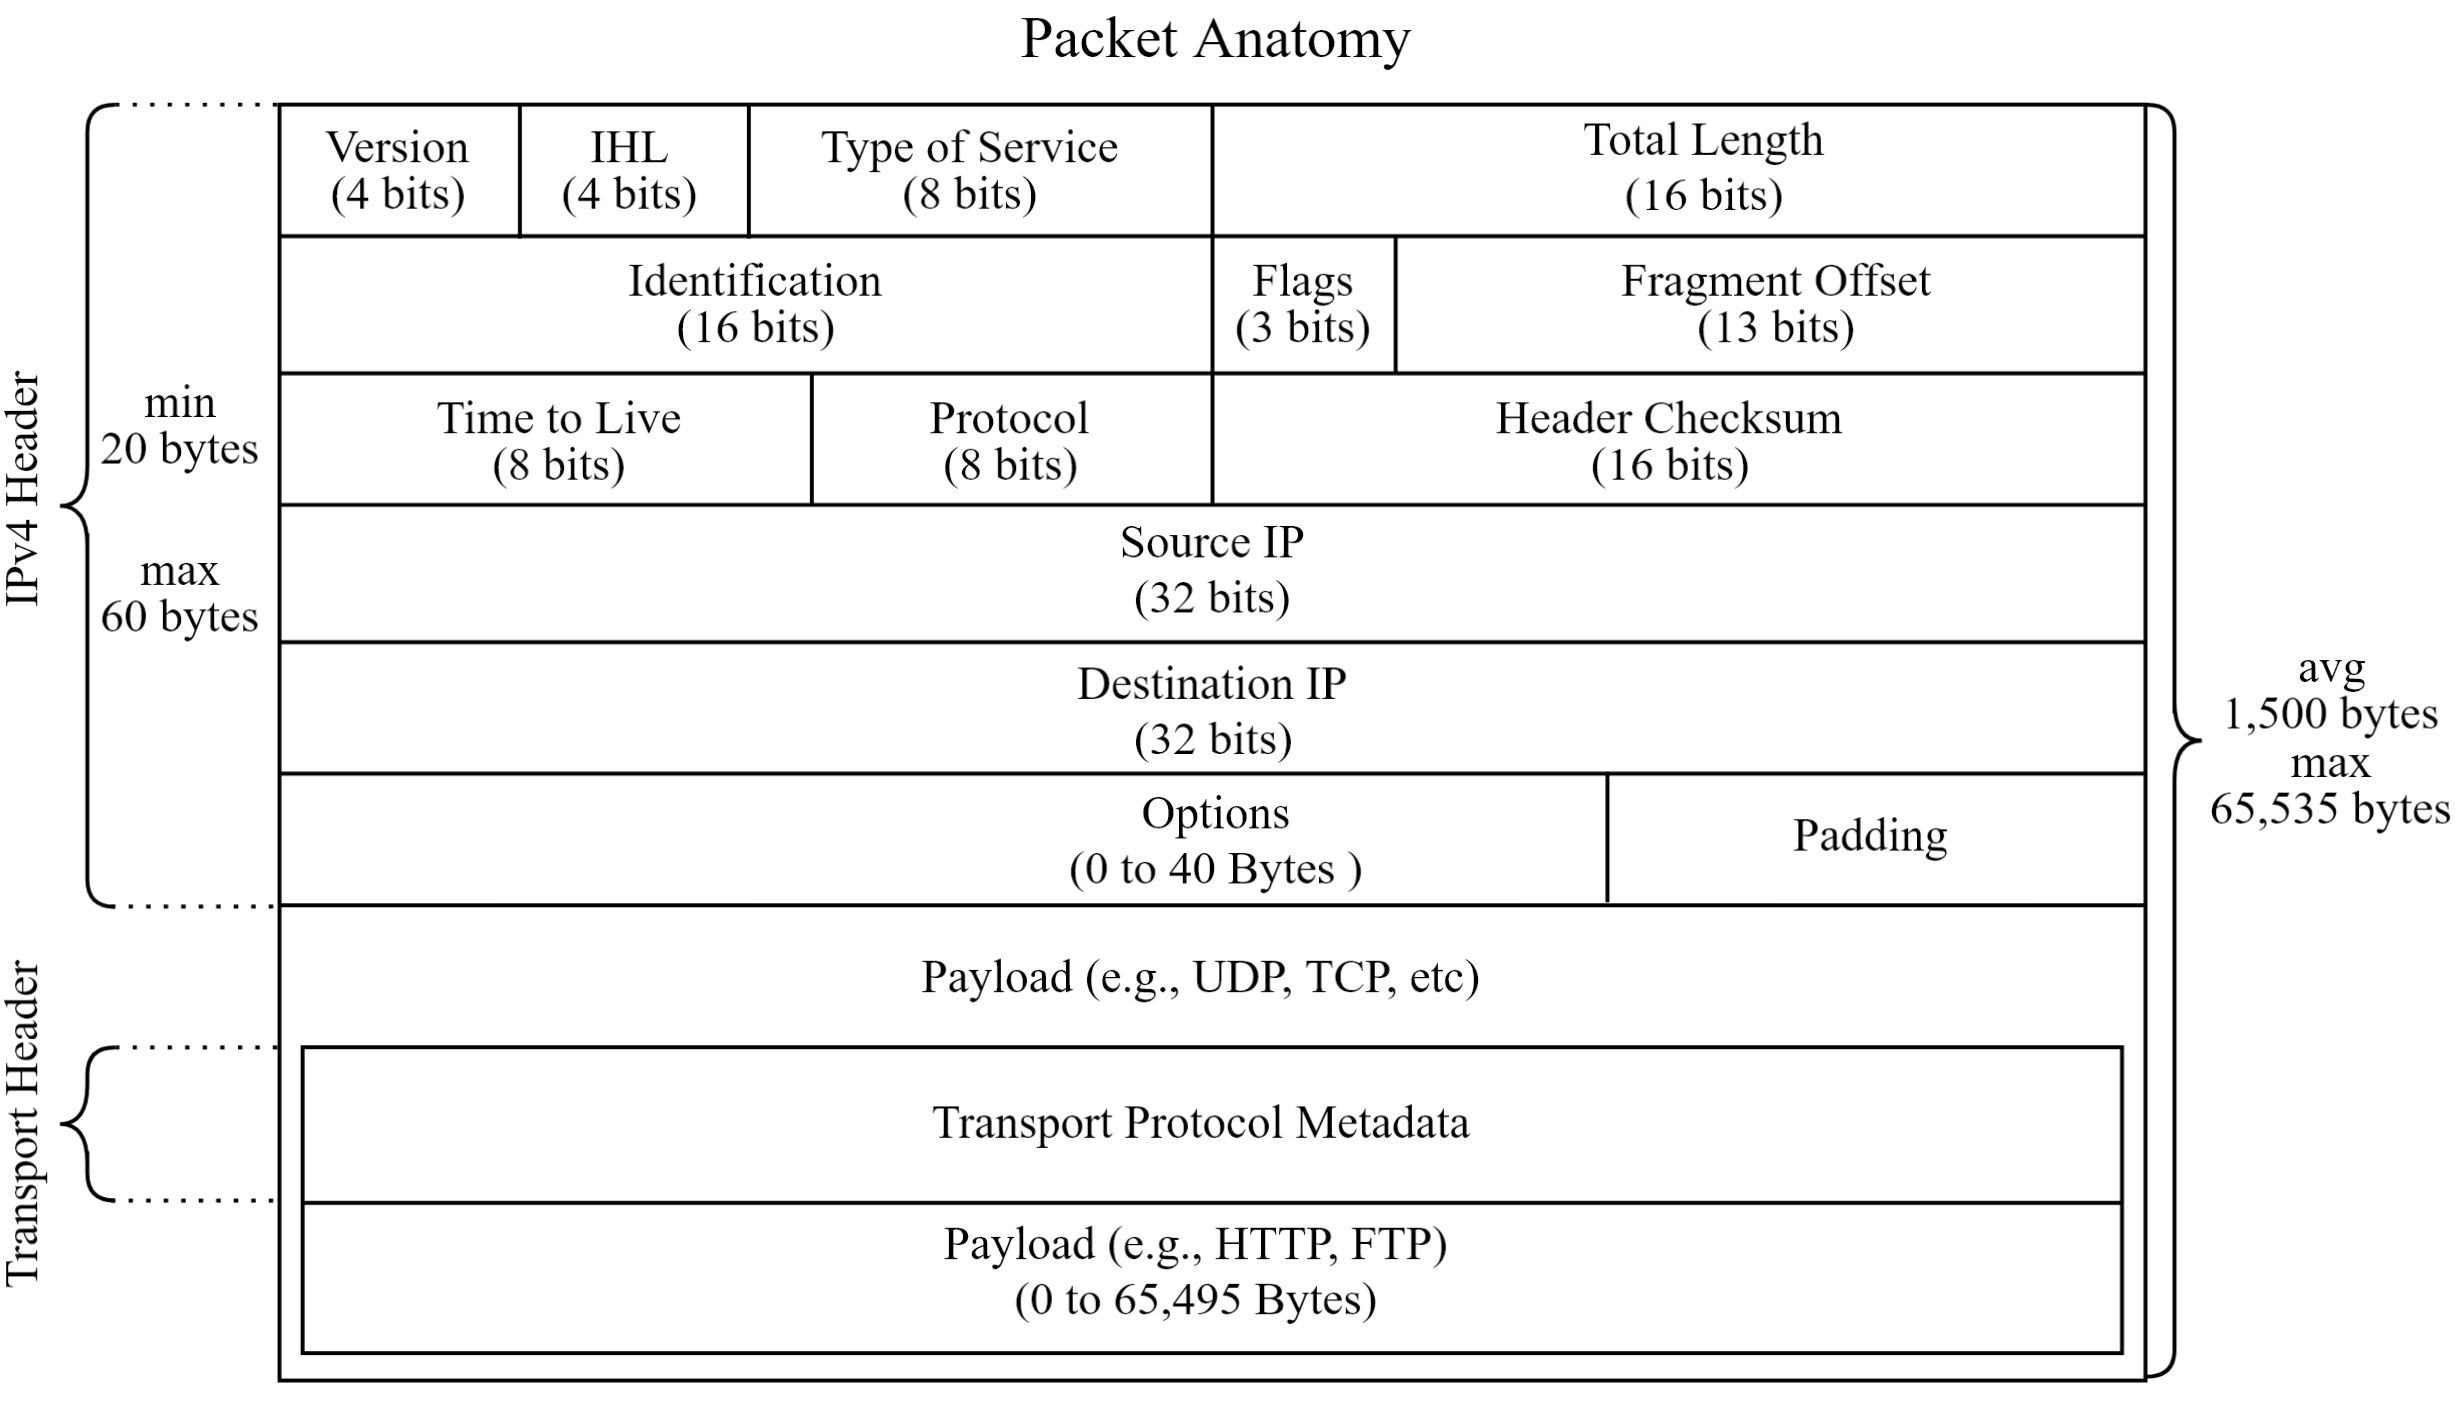
\includegraphics[width=1.1\textwidth]{Sections/network/packet.png}
    \caption{Anatomy of a packet, from IPv4[TCP/UDP[Data]]}
    \label{fig:http}
\end{figure}